\appendix
\section*{\begin{center}{\Huge Appendix}\end{center}}
\addcontentsline{toc}{chapter}{Appendix}
% $\\[0.5cm]$


\chapter{Pseudocode} % (fold)
\label{cha:pseudocode}
\clearpage




\section{Floyd-Warshall Pseudocode} % (fold)
\label{sec:floyd_warshall_pseudocode}

% section floyd_warshall_pseudocode (end)

\begin{algorithm}[H]
\caption{Floyd-Warshall}\label{floyd-warshall-pseudocode}
\begin{algorithmic}[1]

\Procedure{Floyd-Warshall}{Graph}
	\State \textbf{let} $numberOfElements \leftarrow \sum (|N|+|E|+|A|) \in Graph$
	\State \textbf{let} $distances$ be a $numberOfElements \times numberOfElements$ array
	\State \textbf{let} $successors$ be a $numberOfElements \times numberOfElements$ array
	\State \textbf{set} all entries in $distances$ \textbf{to} $\infty$
	\State \textbf{set} all entries in $successors$ \textbf{to} $-1$
	\Statex
	\For{\textbf{each} element $e \in N \cup E \cup A \in Graph$}
		\State $distances[e][e] \leftarrow 0$
		\State $successors[e][e] \leftarrow e$
	\EndFor
	\Statex
	\For{\textbf{each} element $e \in N \cup E \cup A \in Graph$}
		\State \textbf{let} $adjacent \leftarrow $ elements adjacent to $e$ in $Graph$
		\For{\textbf{each} element $e_a \in adjacent$}
			\State $distances[e][e_a] \leftarrow e_a.passThroughCost$
			\State $successors[e][e_a] \leftarrow e_a$
			\State $successors[e_a][e] \leftarrow e$
		\EndFor
	\EndFor
	\Statex
	\For{$k \leftarrow 0$ \textbf{to} $numberOfElements$}
		\For{$i \leftarrow 0$ \textbf{to} $numberOfElements$}
			\For{$j \leftarrow 0$ \textbf{to} $numberOfElements$}
				\If{$distances[i][j] > distances[i][k] + distances[k][j]$}
					\State $distances[i][j] = distances[i][k] + distances[k][j]$
					\State $successors[i][j] = successors[i][k]$
				\EndIf
			\EndFor
		\EndFor
	\EndFor
	\Statex
	\For{\textbf{each} element $(e_i,e_j) \in N \cup E \cup A \in Graph$}
		\If{$e_i \neq e_j$}
			\State $distances[e_j][e_i] \leftarrow distances[e_j][e_i] - e_i.passThroughCost$
		\EndIf
	\EndFor
\EndProcedure

\end{algorithmic}
\end{algorithm}


\section{Split Pseudocode} % (fold)
\label{sec:split_pseudocode}

% section split_pseudocode (end)

\begin{algorithm}[H]
\caption{Split}\label{split-pseudocode}
\begin{algorithmic}[1]

\Procedure{Split}{Genotype,Graph,Distances}
	\State \textbf{let} $numberOfElements \leftarrow \sum (|N|+|E|+|A|) \in Graph$
	\State \textbf{let} $e_k$ be the k'th element from the Genotypes ordering of the set $(N \cup E \cup A) \in Graph$ in its genome
	\State \textbf{let} $costs$ be an array of length $numberOfElements + 1$
	\State \textbf{let} $predecessors$ be an array of length $numberOfElements + 1$
	\State \textbf{set} all entries in $costs$ to $\infty$
	\State $costs[0] \leftarrow 0$
	\State $predecessors[0] \leftarrow 0$
	\Statex
	\For{$i \leftarrow 1$ \textbf{to} $numberOfElements + 1$}
		\State $j \leftarrow i$
		\State $load \leftarrow 0$
		\State $cost \leftarrow 0$
		\DoWhile
			\State $load \leftarrow load + e_j.demand$
			\Statex
			\If{$i = j$}
				\State $cost \leftarrow($ distance from depot to $e_{i-1}) + e_{i-1}.servicing\_cost +($ distance from $e_{i-1}$ to the depot $)$
			\Else
				\State $cost \leftarrow  cost - ($ distance from $e_{j-2}$ to depot $) + ($distance from $e_{j-2}$ to $e_{j-1}) + e_{j-1}.servicing\_cost +($ distance from $e_{j-1}$ to the depot $)$
			\EndIf
			\Statex
			\If{$(load < vehicle\_capacity)\wedge(costs[i - 1] + cost < costs[j])$}
				\State $costs[j] \leftarrow costs[i - 1] + cost$
				\State $predecessors[j] \leftarrow i - 1$
			\EndIf
			\Statex
			\State $j \leftarrow j + 1$
		\EndDoWhile{$(j < numberOfElements + 1)\wedge(load < vehicle\_capacity)$}
	\EndFor
	\Statex
	\State \textbf{let} $Genotype.fitness \leftarrow costs[last\_index]$
\EndProcedure

\end{algorithmic}
\end{algorithm}


\section{Split Retrieve Trips Pseudocode} % (fold)
\label{sec:split_retrieve_trips_pseudocode}

% section split_retrieve_trips_pseudocode (end)

\begin{algorithm}[H]
\caption{Retrieve Trips from Split}\label{split-retrieve-pseudocode}
\begin{algorithmic}[1]

\Procedure{Retrieve Trips From Split}{predecessors, genotype}
	\State \textbf{let} $list\_of\_trips$ be an empty list
	\State $j \leftarrow$ number of tasks
	\DoWhile
		\State $i \leftarrow predecessors[j]$
		\State \textbf{let} $current\_trip$ be a new array of size $j - i$
		\For{$k \leftarrow i + 1$ \textbf{to} $k \leq j$, $k \leftarrow k + 1$}
			\State $current\_trip[k-(i+1)] \leftarrow genotype.genome[k-1]$
		\EndFor
		\State \textbf{add} $current\_trip$ \textbf{to} the beginning of $list\_of\_trips$
		\State $j \leftarrow i$
	\EndDoWhile{$i \neq 0$}
\EndProcedure

\end{algorithmic}
\end{algorithm}

% chapter pseudocode (end)


\chapter{Memetic Algorithm Tuning Results} % (fold)
\label{cha:memetic_algorithm_tunin_results}

\section{Population Size Testing Results} % (fold)
\label{sec:population_size_testing_results}

\begin{landscape}
\begin{figure}[thbp]
	\centerline{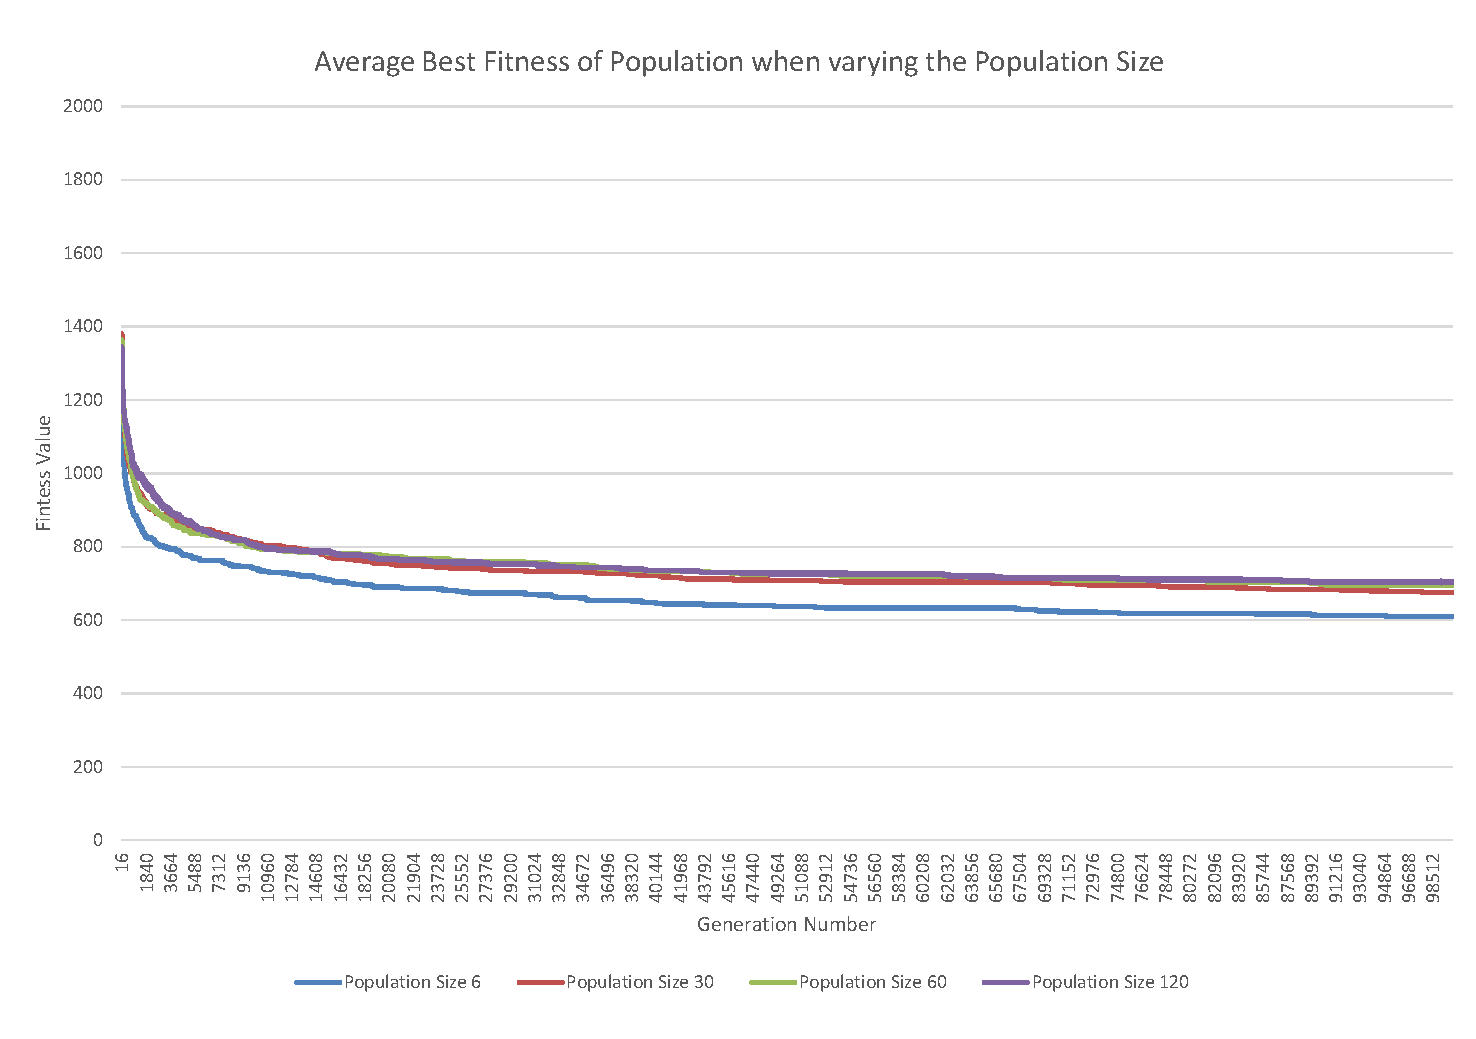
\includegraphics[height=0.945\textwidth]{figures/CircleTests/PopulationSize/CircleTestsPopulationAverageBest.pdf}}
	\caption{Population Size - Average Best}
	\label{fig:ctpab}
\end{figure}
\end{landscape}

\begin{landscape}
\begin{figure}[thbp]
	\centerline{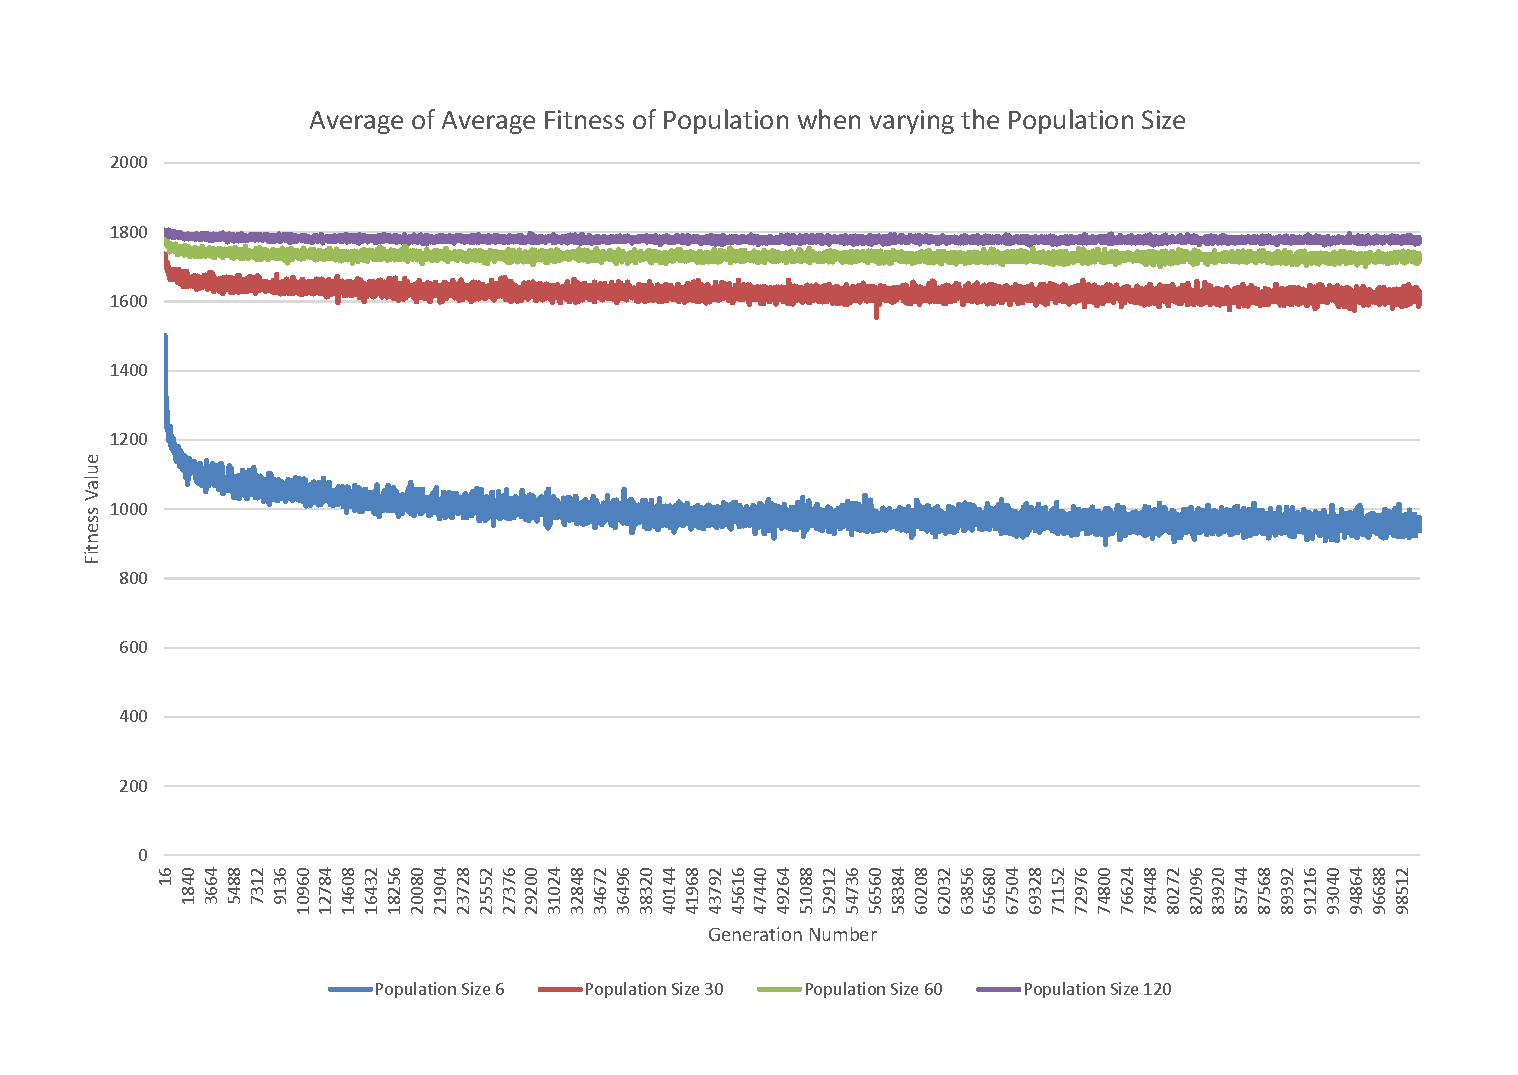
\includegraphics[height=0.945\textwidth]{figures/CircleTests/PopulationSize/CircleTestsPopulationAverageAverage.pdf}}
	\caption{Population Size - Average Average}
\end{figure}
\end{landscape}

\begin{landscape}
\begin{figure}[thbp]
	\centerline{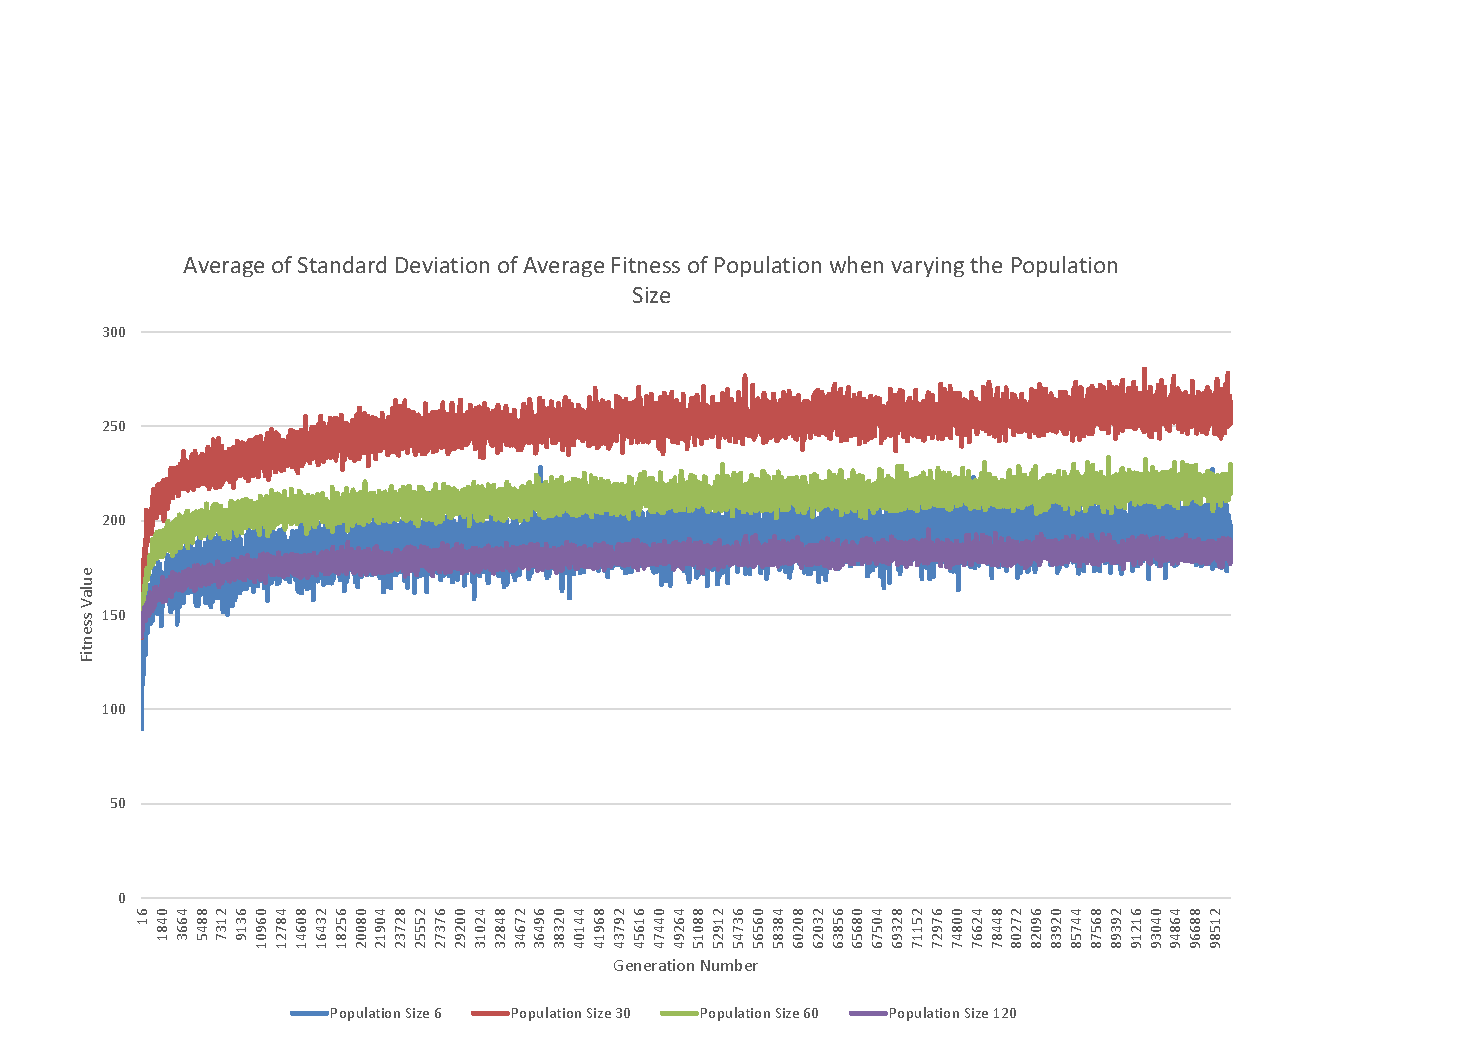
\includegraphics[height=0.945\textwidth]{figures/CircleTests/PopulationSize/CircleTestsPopulationAverageStandardDeviation.pdf}}
	\caption{Population Size - Average Standard Deviation}
\end{figure}
\end{landscape}

% section population_size_testing_results (end)

\section{Parent Selection Results} % (fold)
\label{sec:parent_selection_results}

\begin{landscape}
\begin{figure}[thbp]
	\centerline{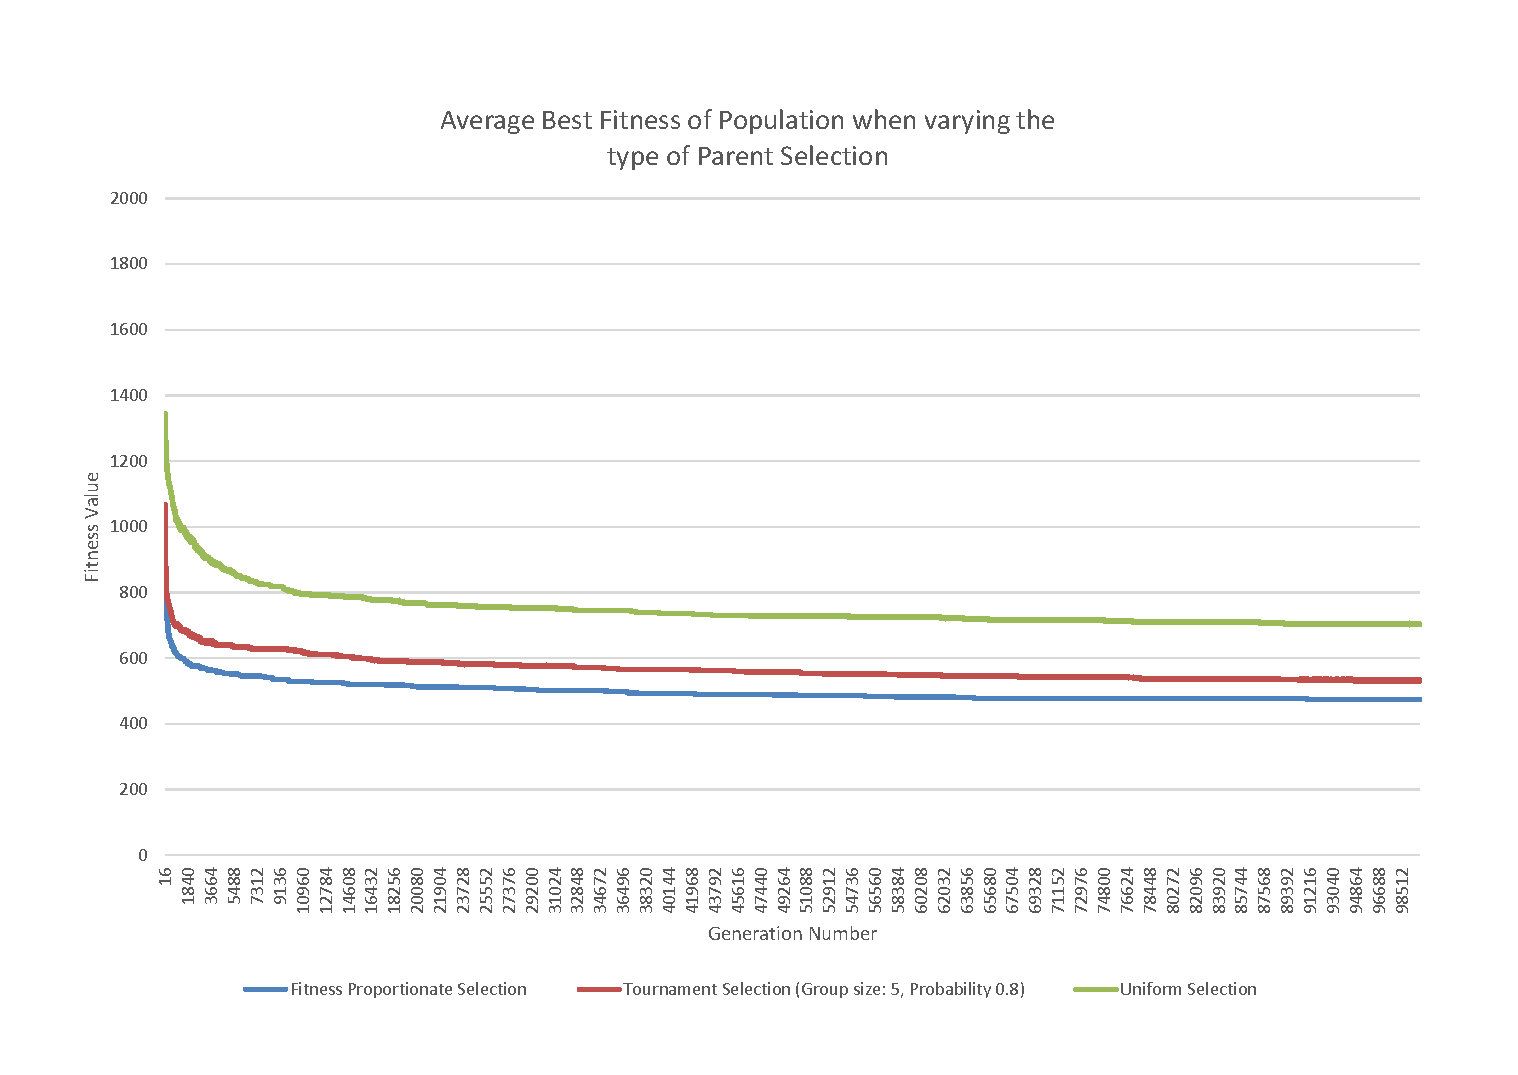
\includegraphics[height=0.945\textwidth]{figures/CircleTests/ParentSelection/CircleTestParentSelectionAverageBest.pdf}}
	\caption{Parent Selection - Average Best}
	\label{fig:ctpsab}
\end{figure}
\end{landscape}

\begin{landscape}
\begin{figure}[thbp]
	\centerline{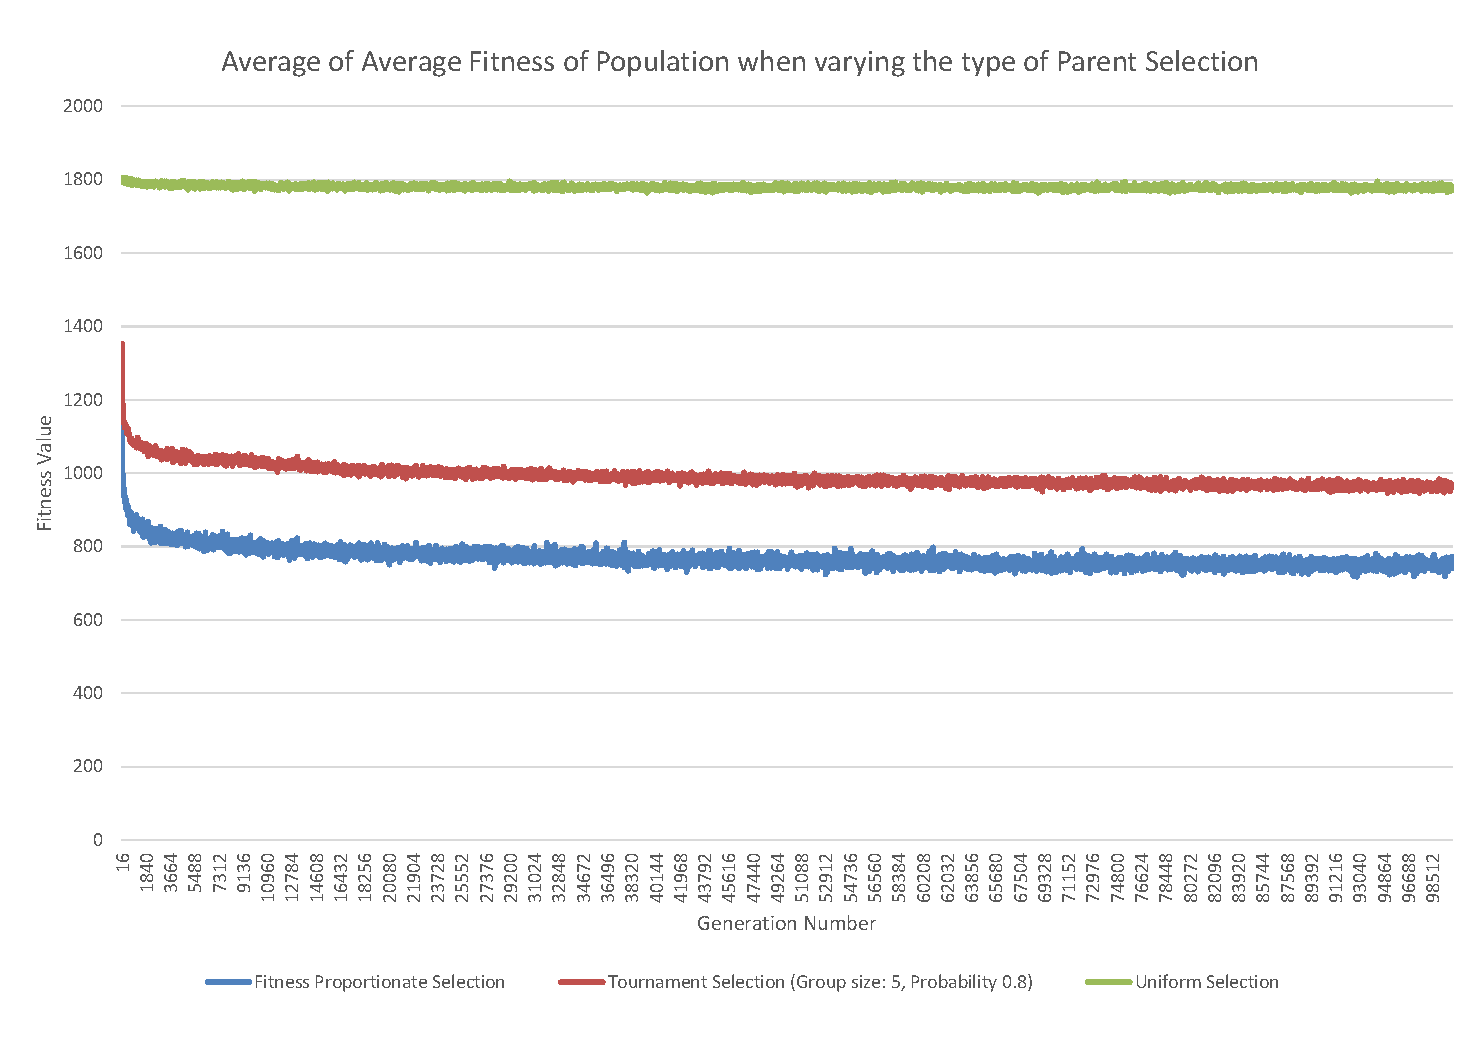
\includegraphics[height=0.945\textwidth]{figures/CircleTests/ParentSelection/CircleTestParentSelectionAverageAverage.pdf}}
	\caption{Parent Selection - Average Average}
\end{figure}
\end{landscape}

\begin{landscape}
\begin{figure}[thbp]
	\centerline{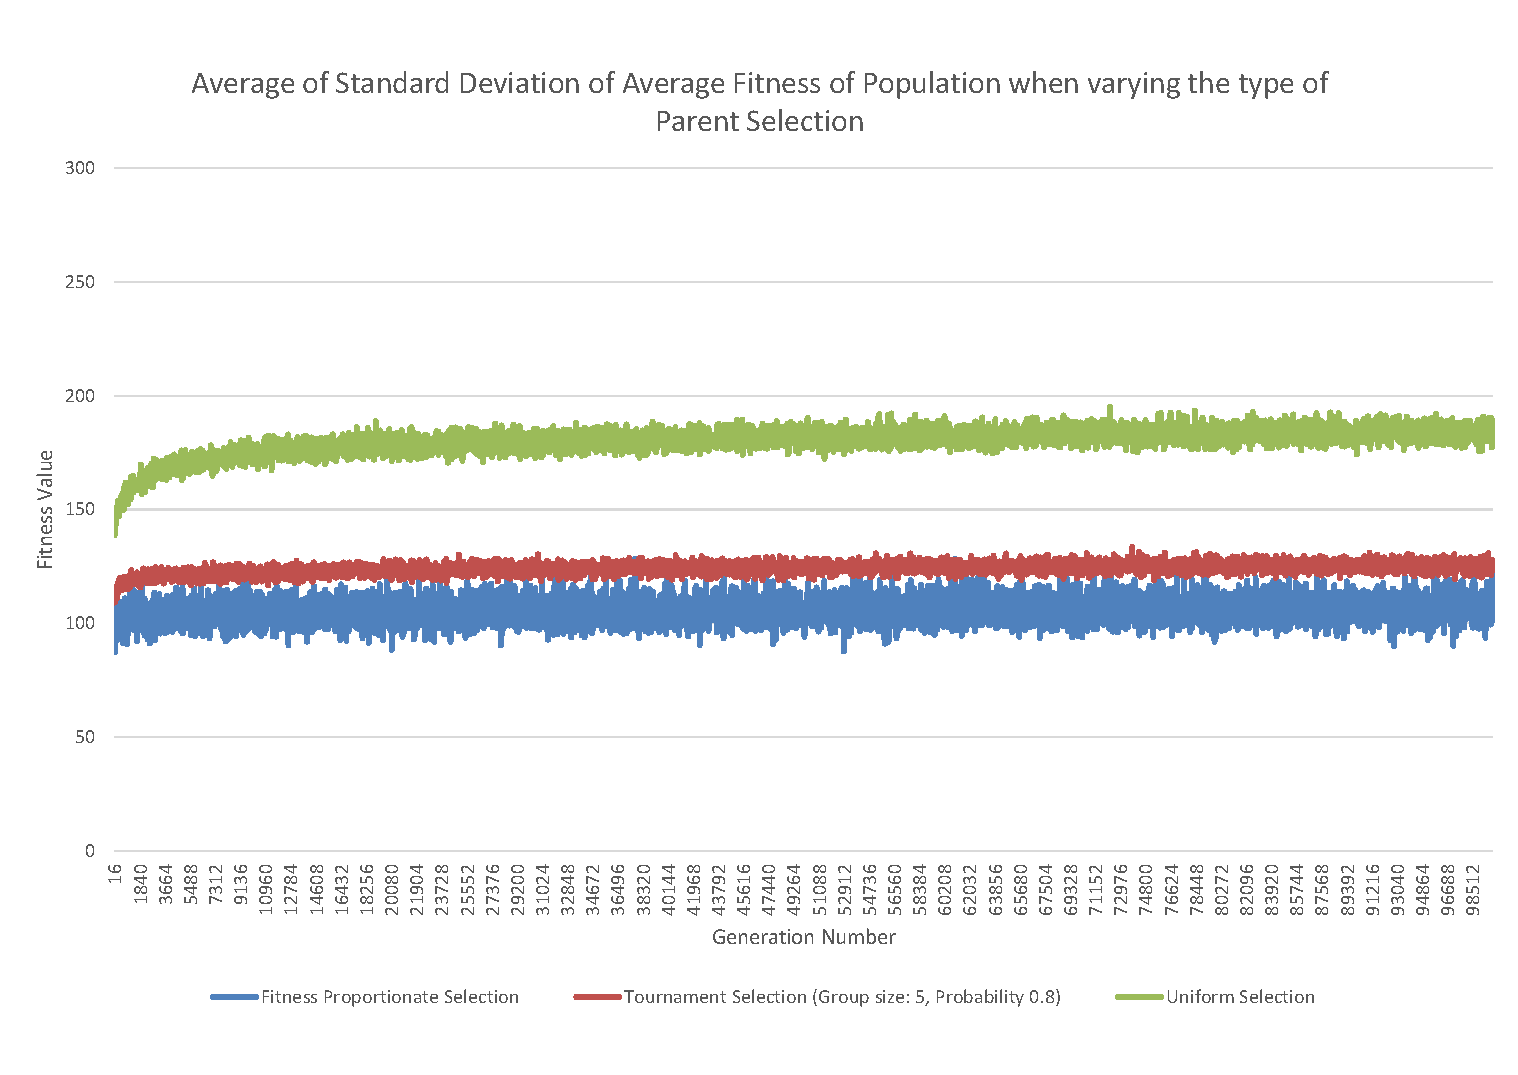
\includegraphics[height=0.945\textwidth]{figures/CircleTests/ParentSelection/CircleTestParentSelectionAverageStandardDeviation.pdf}}
	\caption{Parent Selection - Average Standard Deviation}
\end{figure}
\end{landscape}

% section parent_selection_results (end)

\section{Adult Selection Results} % (fold)
\label{sec:adult_selection_results}

\begin{landscape}
\begin{figure}[thbp]
	\centerline{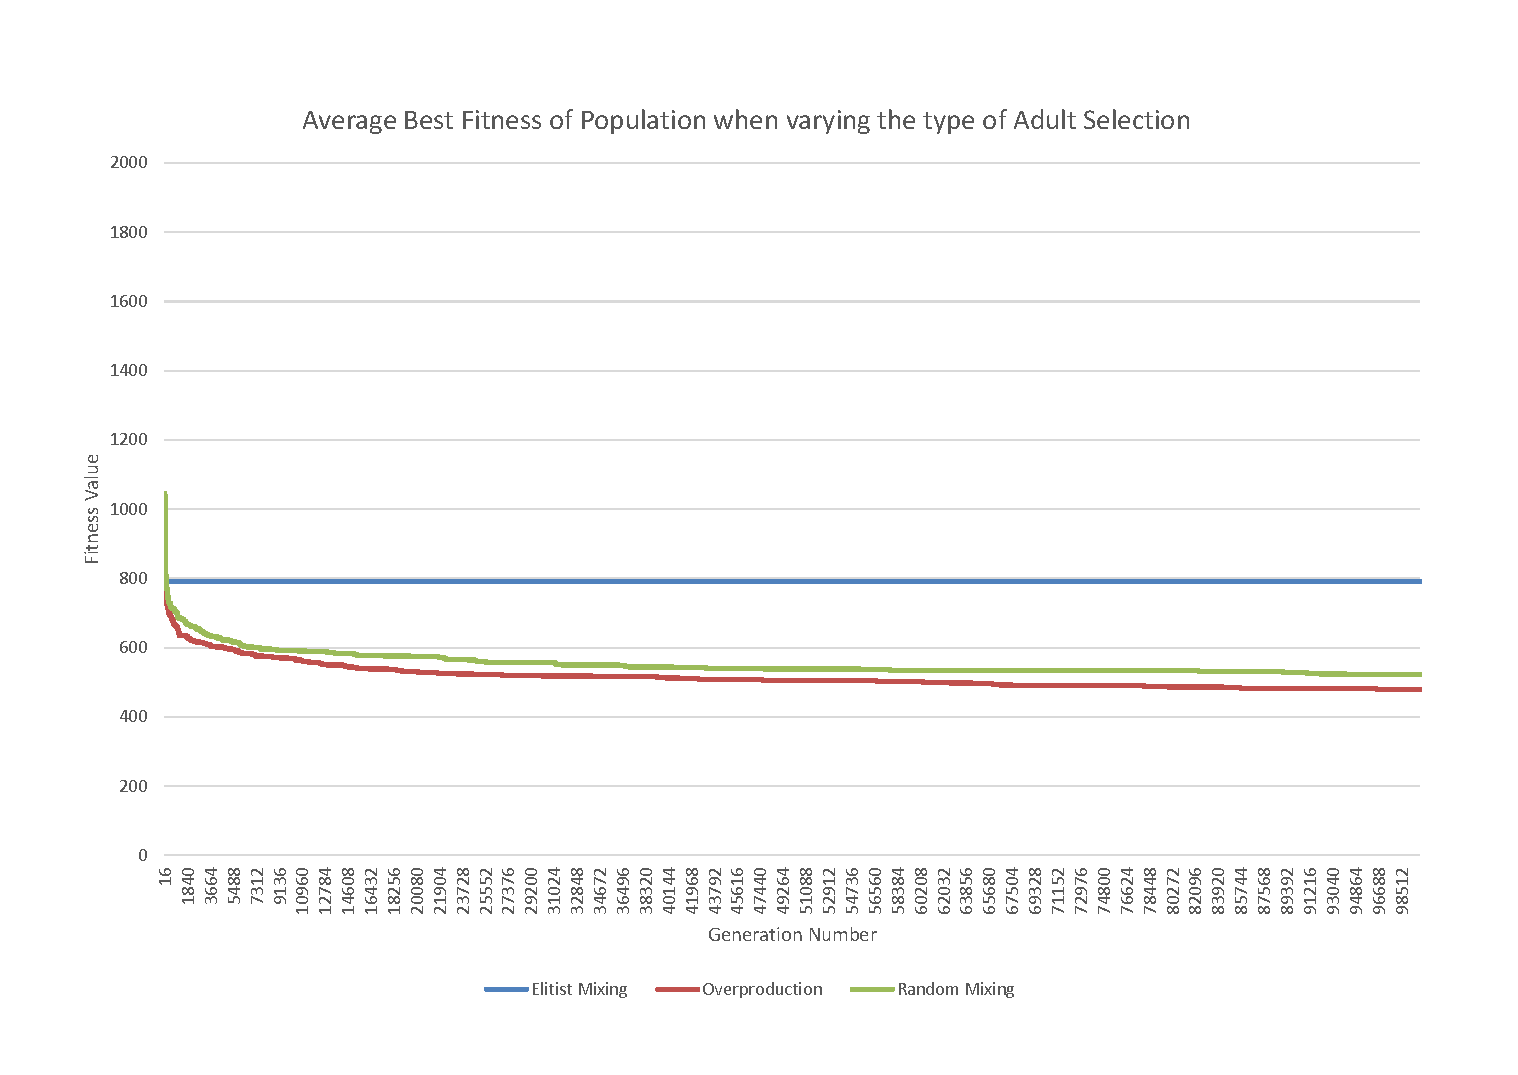
\includegraphics[height=0.945\textwidth]{figures/CircleTests/AdultSelection/CircleTestAdultSelectionAverageBest.pdf}}
	\caption{Adult Selection - Average Best}
	\label{fig:ctasab}
\end{figure}
\end{landscape}

\begin{landscape}
\begin{figure}[thbp]
	\centerline{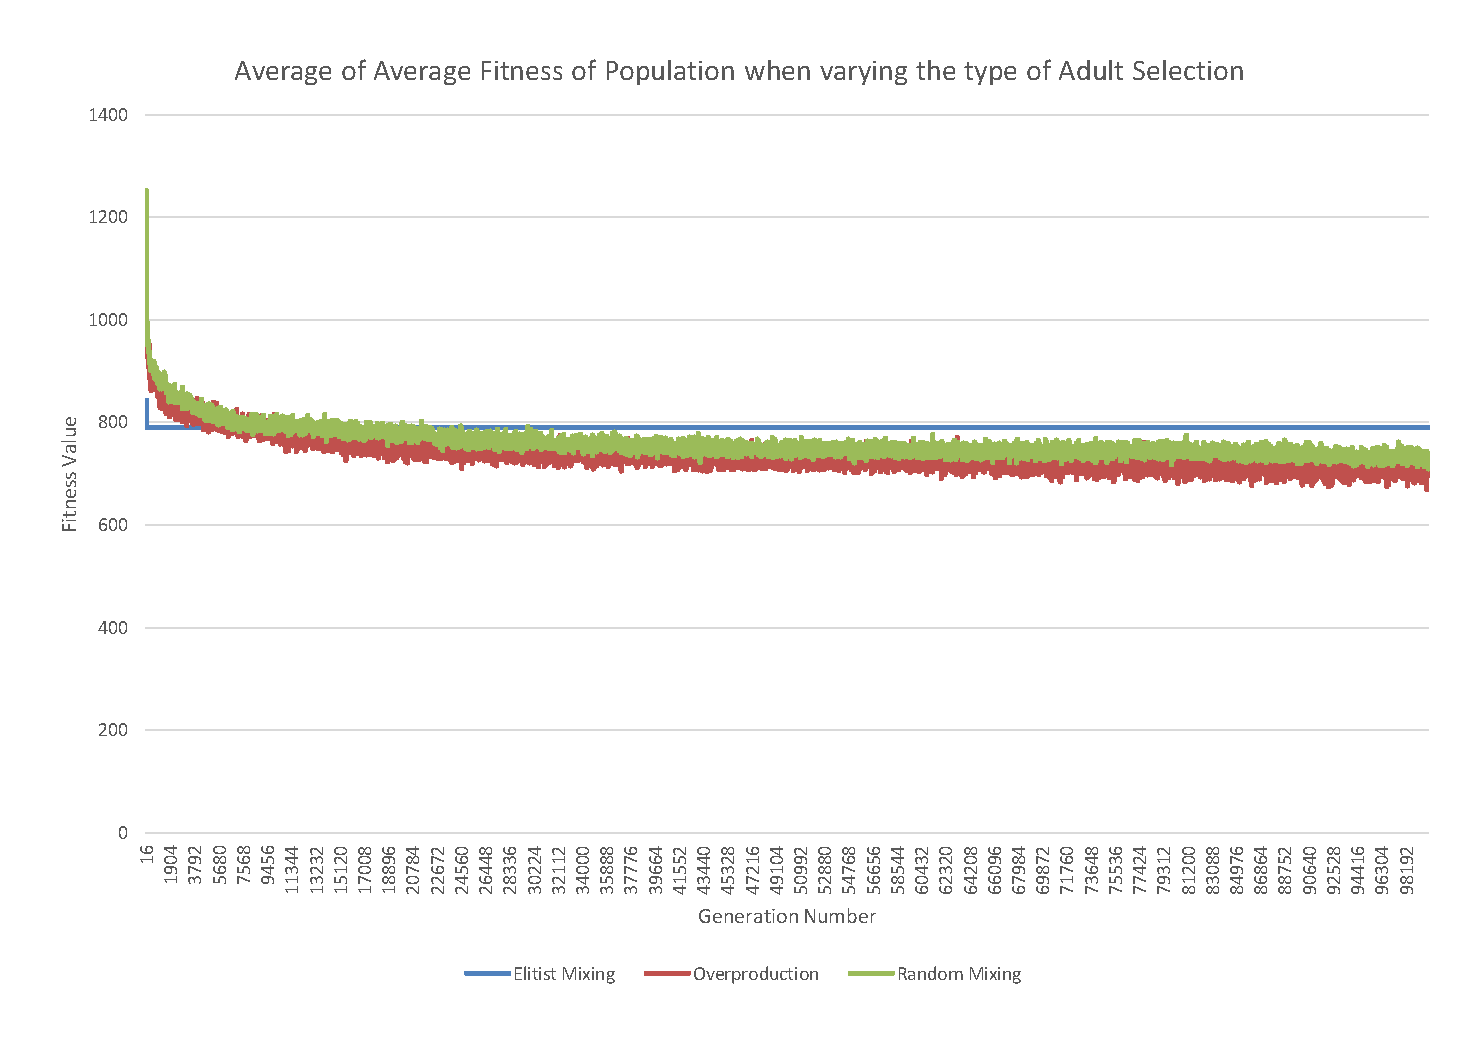
\includegraphics[height=0.945\textwidth]{figures/CircleTests/AdultSelection/CircleTestAdultSelectionAverageAverage.pdf}}
	\caption{Adult Selection - Average Average}
	\label{fig:ctasaa}
\end{figure}
\end{landscape}

\begin{landscape}
\begin{figure}[thbp]
	\centerline{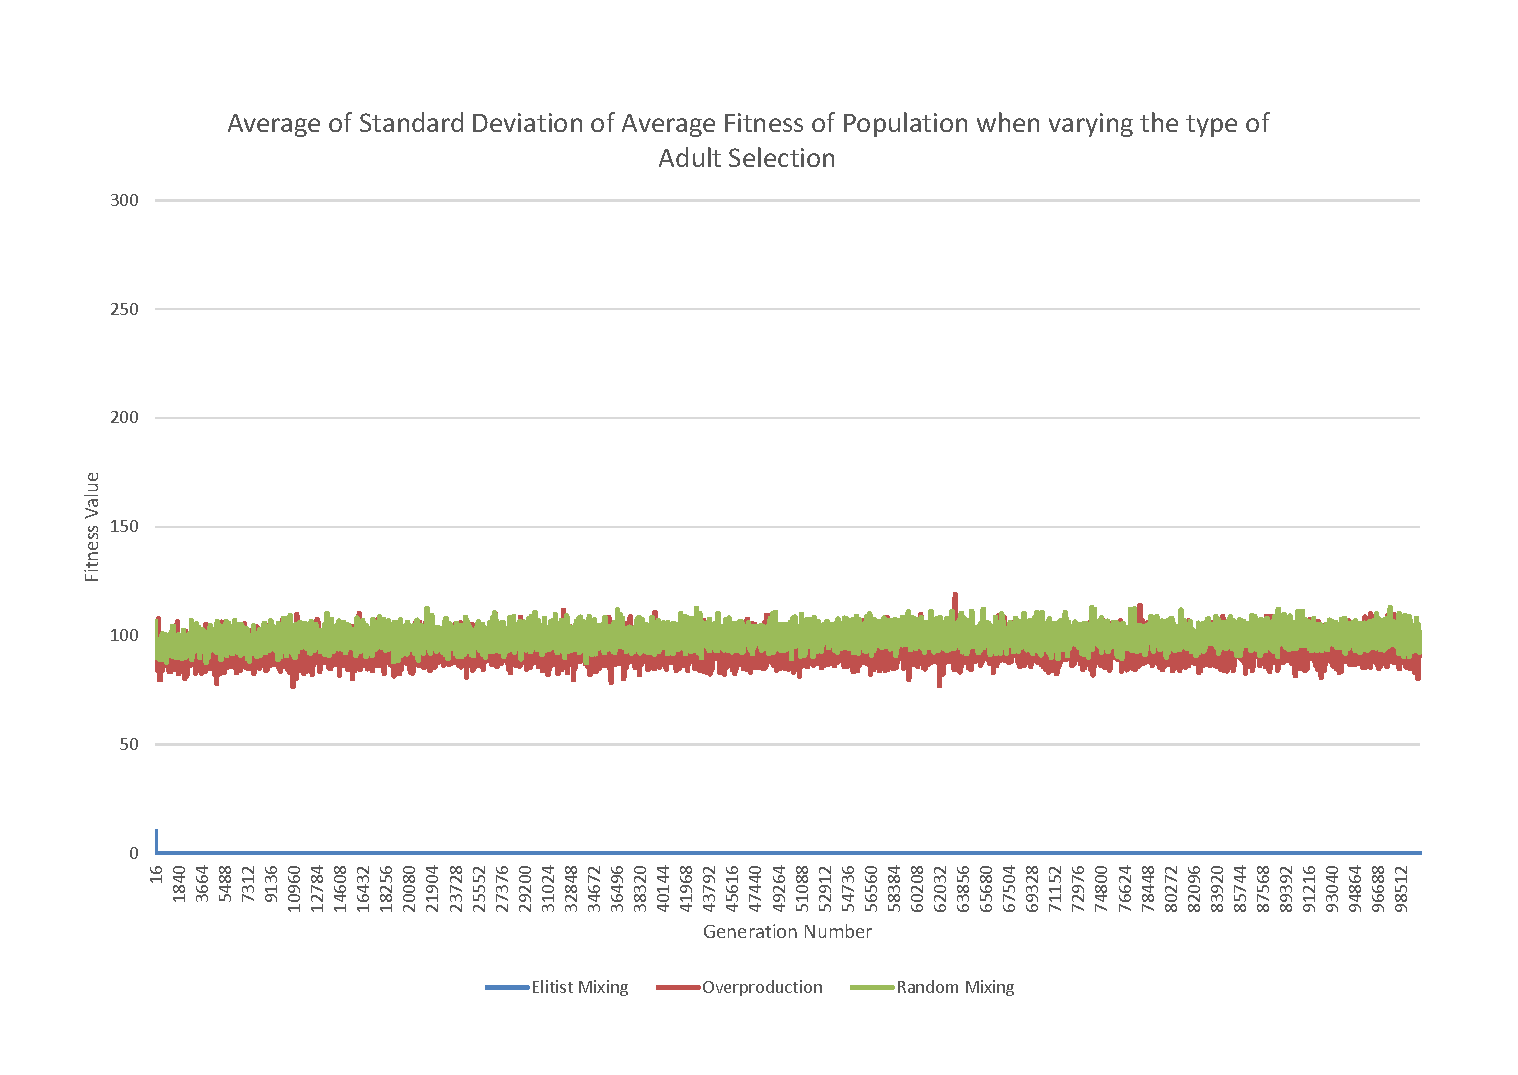
\includegraphics[height=0.945\textwidth]{figures/CircleTests/AdultSelection/CircleTestAdultSelectionAverageStandardDeviation.pdf}}
	\caption{Adult Selection - Average Standard Deviation}
	\label{fig:ctasasd}
\end{figure}
\end{landscape}

% section adult_selection_results (end)

\section{Mutation Types Results} % (fold)
\label{sec:mutation_types_results}

\begin{landscape}
\begin{figure}[thbp]
	\centerline{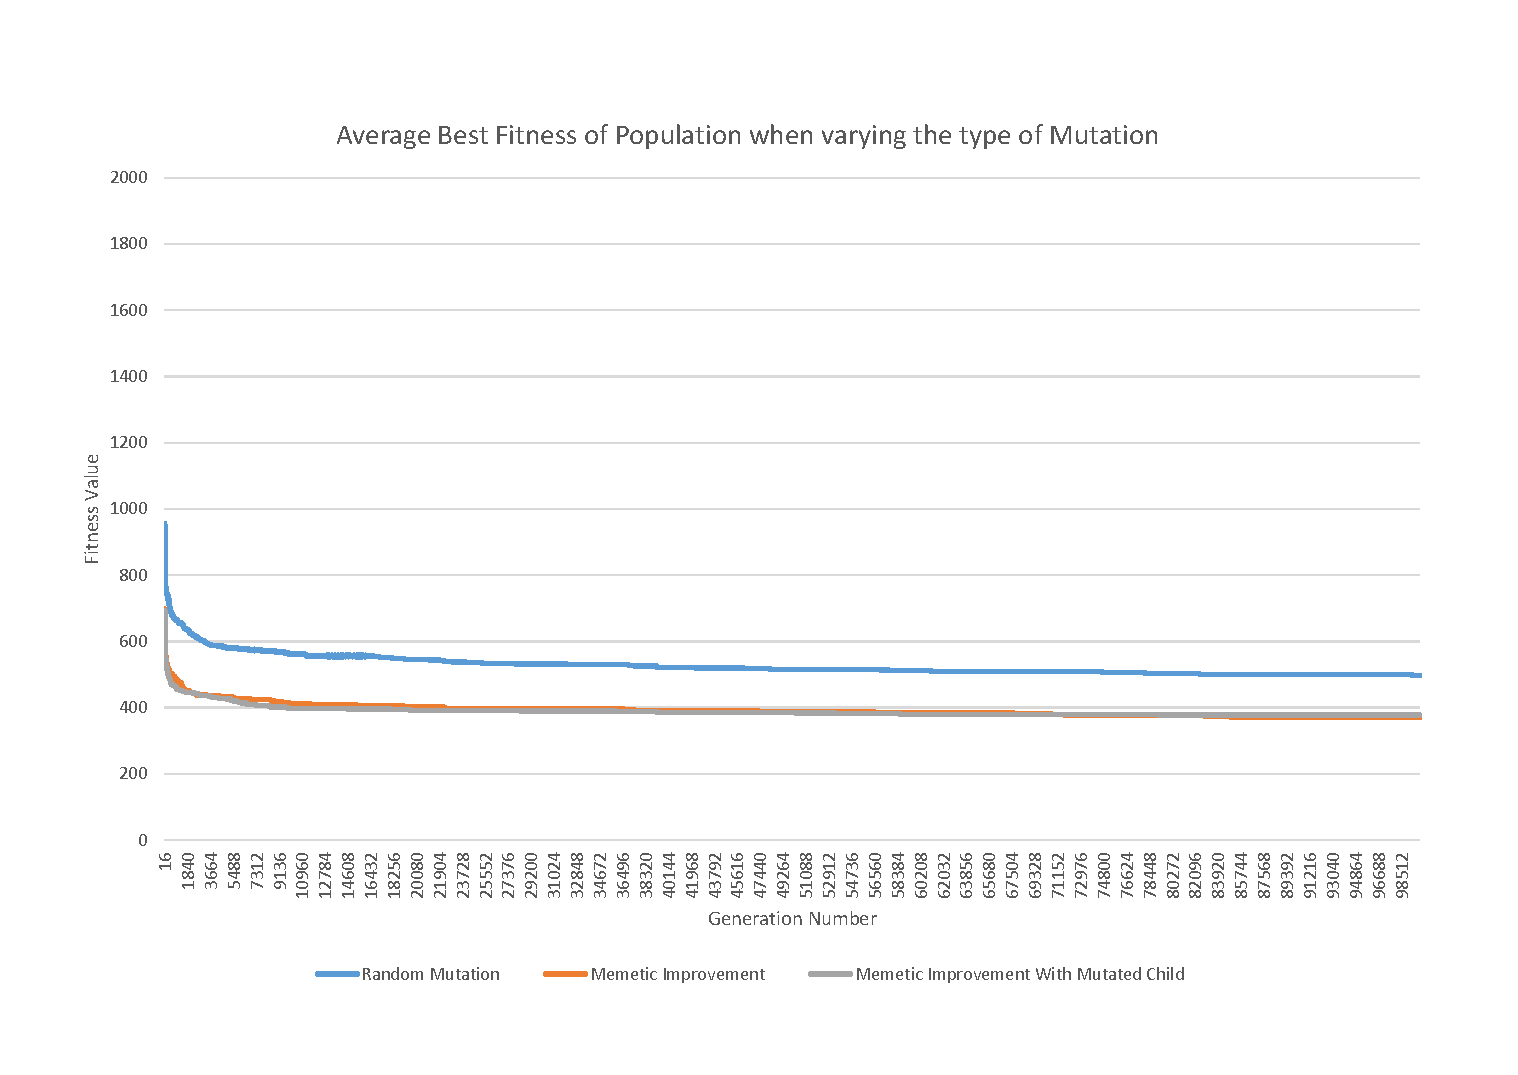
\includegraphics[height=0.945\textwidth]{figures/CircleTests/Mutation/CircleTestMutationAverageBest.pdf}}
	\caption{Mutation - Average Best}
	\label{fig:ctmab}
\end{figure}
\end{landscape}

\begin{landscape}
\begin{figure}[thbp]
	\centerline{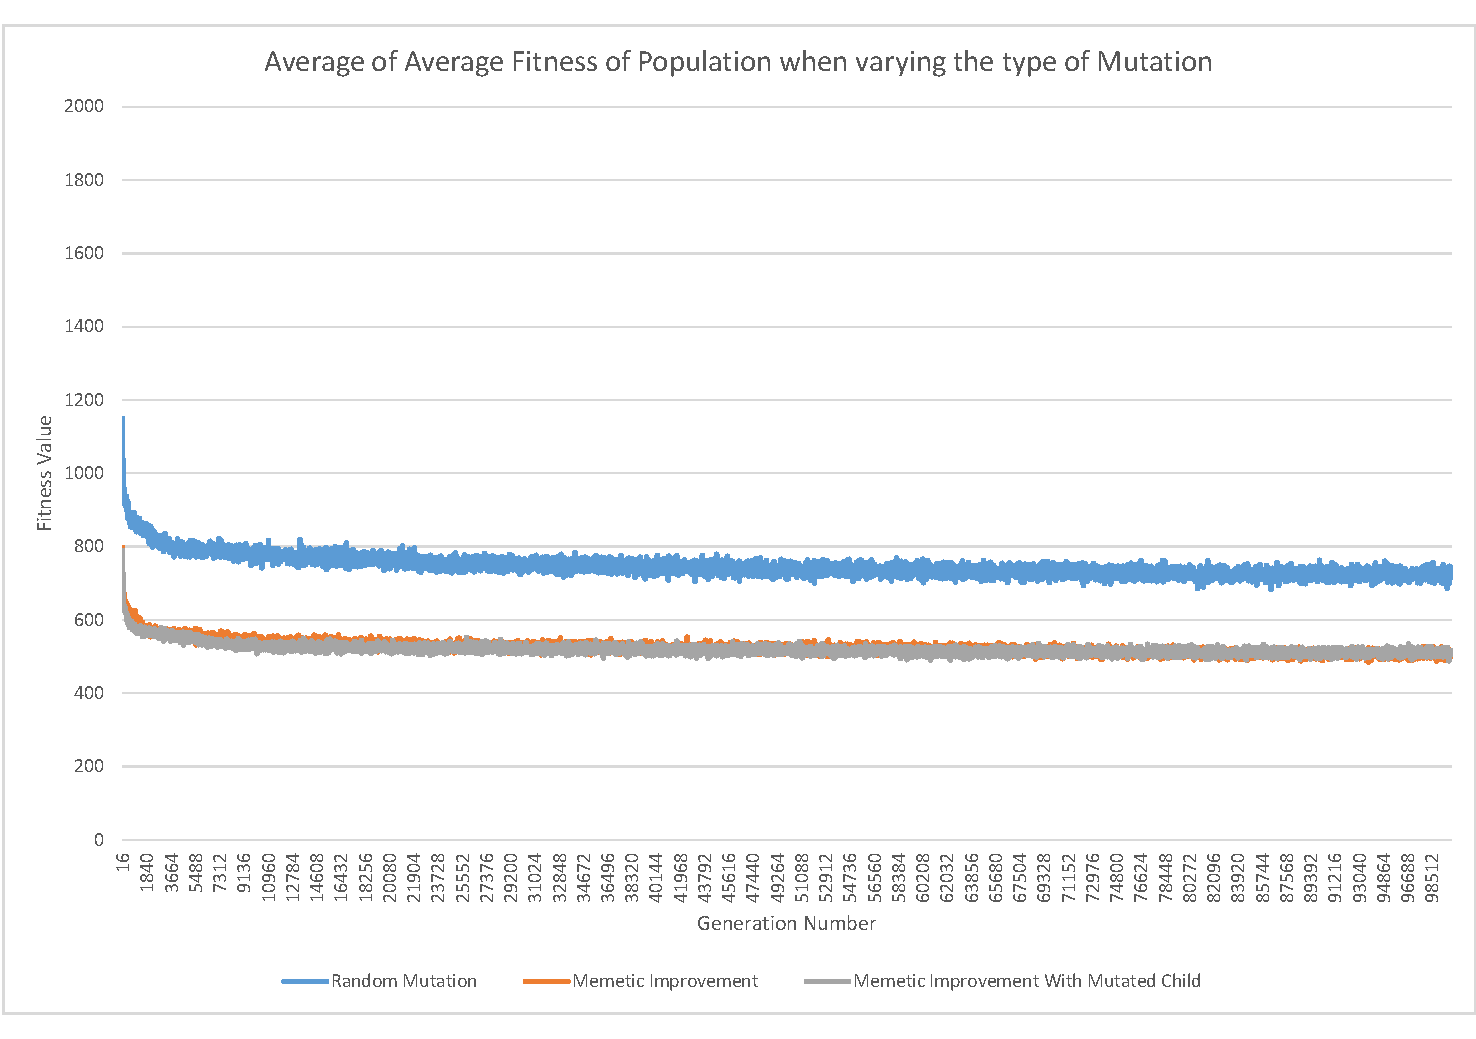
\includegraphics[height=0.945\textwidth]{figures/CircleTests/Mutation/CircleTestMutationAverageAverage.pdf}}
	\caption{Mutation - Average Average}
	\label{fig:ctmaa}
\end{figure}
\end{landscape}

\begin{landscape}
\begin{figure}[thbp]
	\centerline{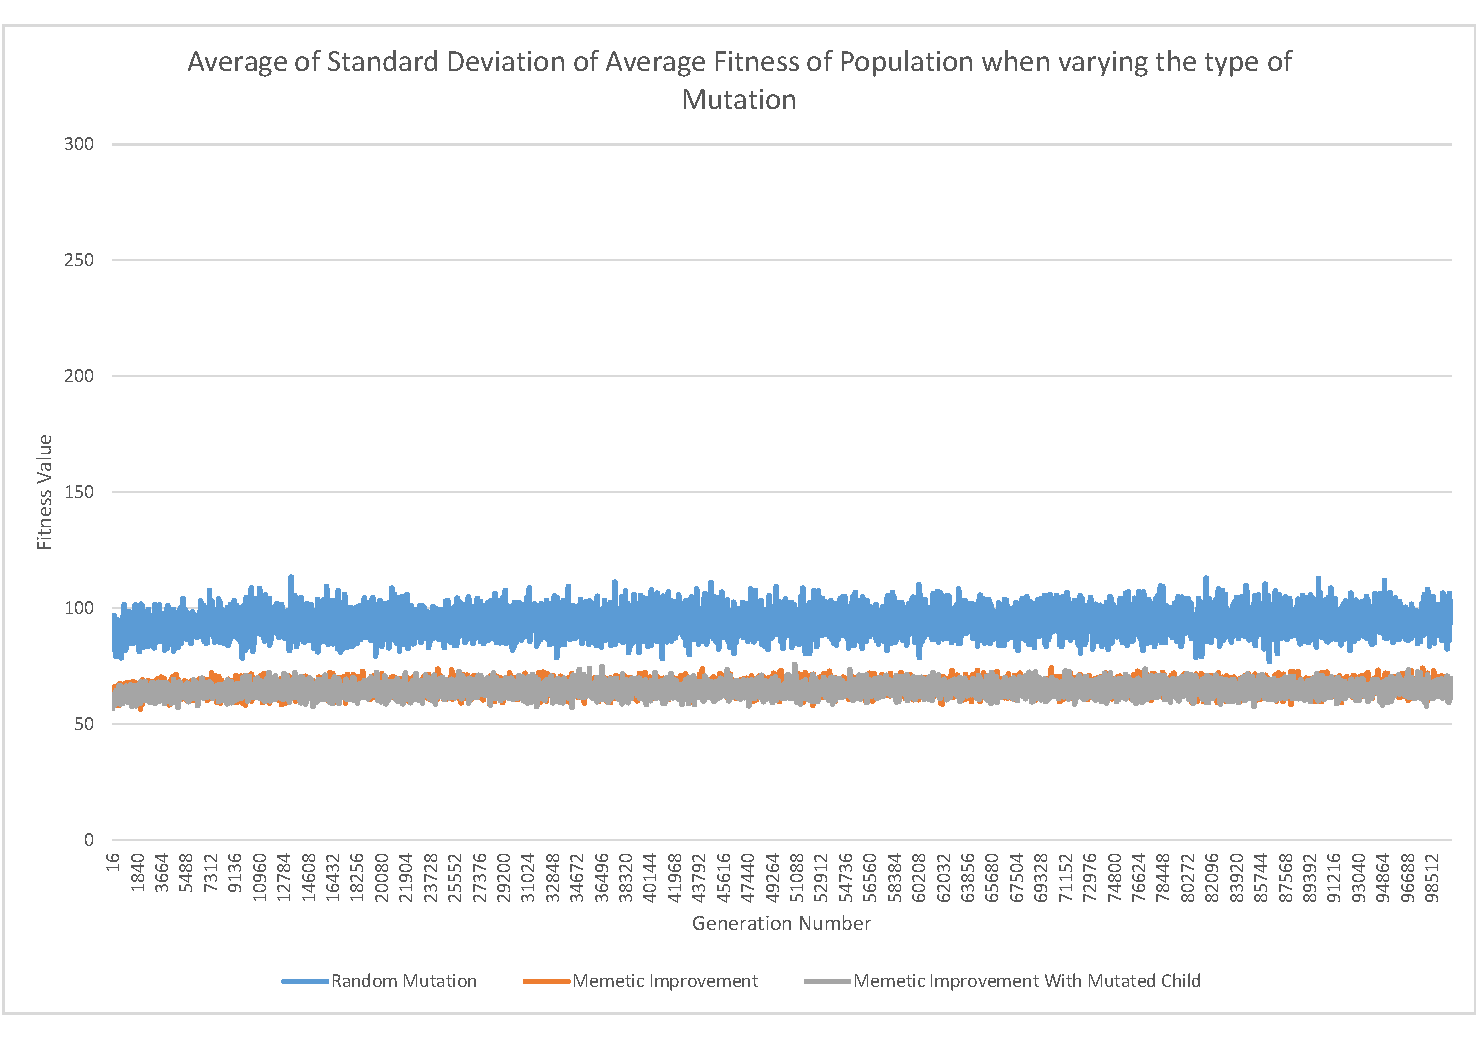
\includegraphics[height=0.945\textwidth]{figures/CircleTests/Mutation/CircleTestMutationAverageStandardDeviation.pdf}}
	\caption{Mutation - Average Standard Deviation}
	\label{fig:ctmasd}
\end{figure}
\end{landscape}

% section mutation_types (end)

\section{Population Size Control Results} % (fold)
\label{sec:population_size_control_results}

\begin{landscape}
\begin{figure}[thbp]
	\centerline{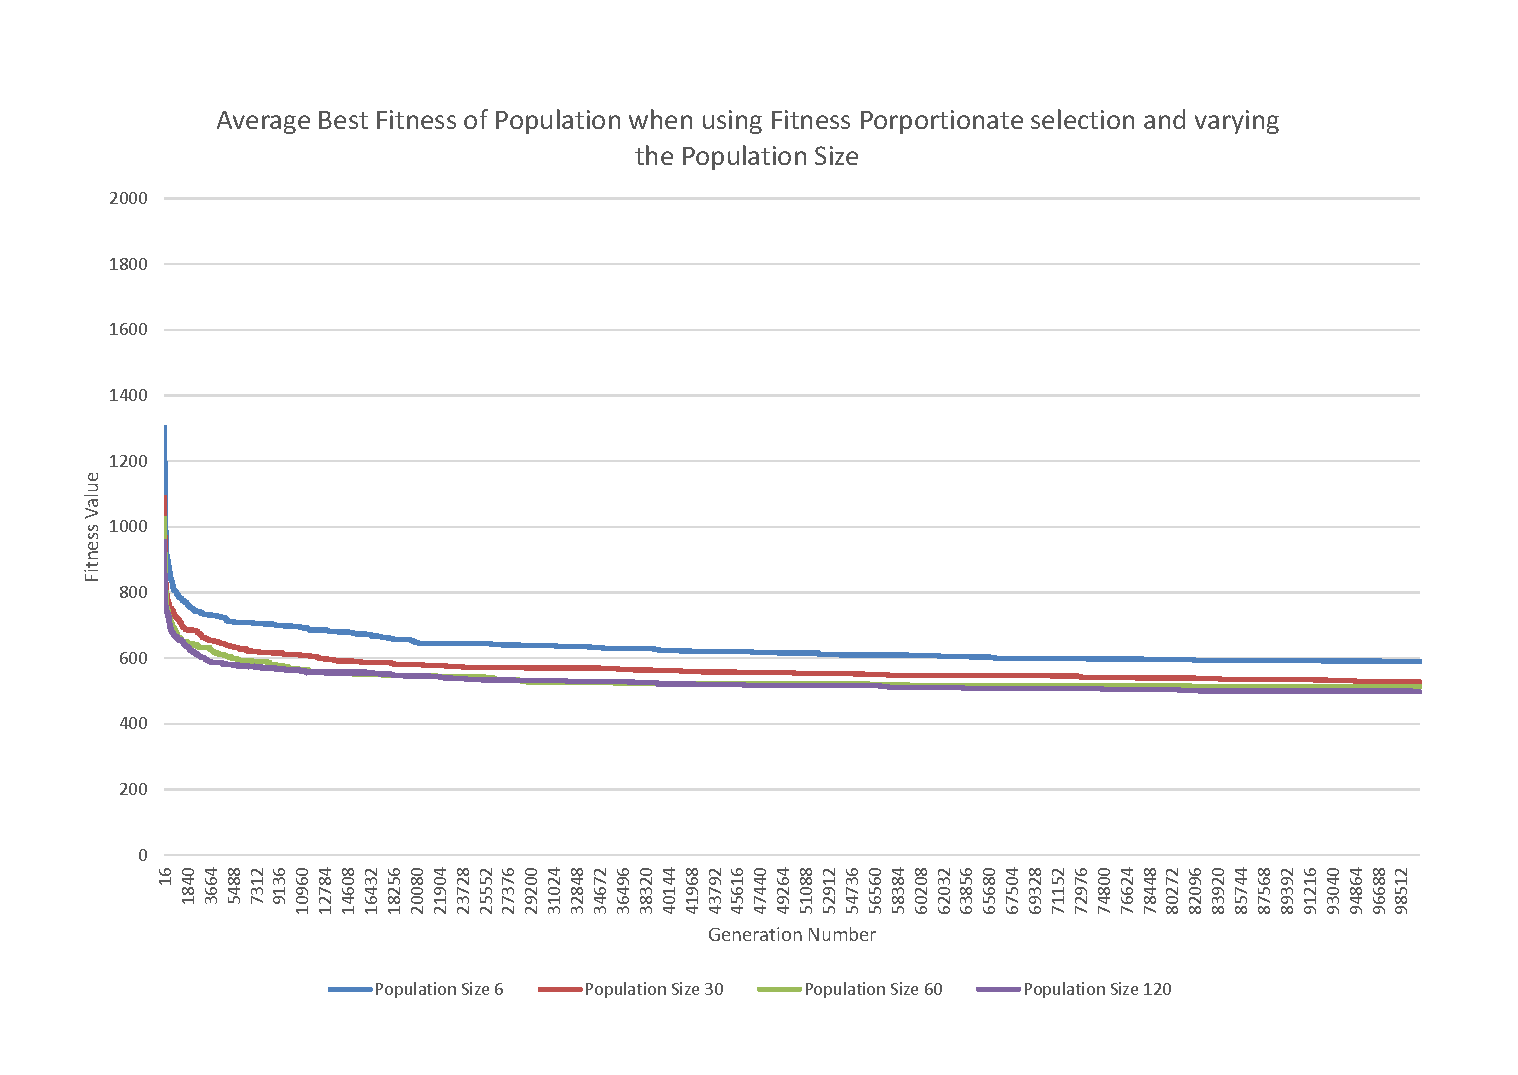
\includegraphics[height=0.945\textwidth]{figures/CircleTests/PopulationSizeControl/CirclePopulationSizeControllAverageBest.pdf}}
	\caption{Population Size Control - Average Best}
	\label{fig:cpscab}
\end{figure}
\end{landscape}

\begin{landscape}
\begin{figure}[thbp]
	\centerline{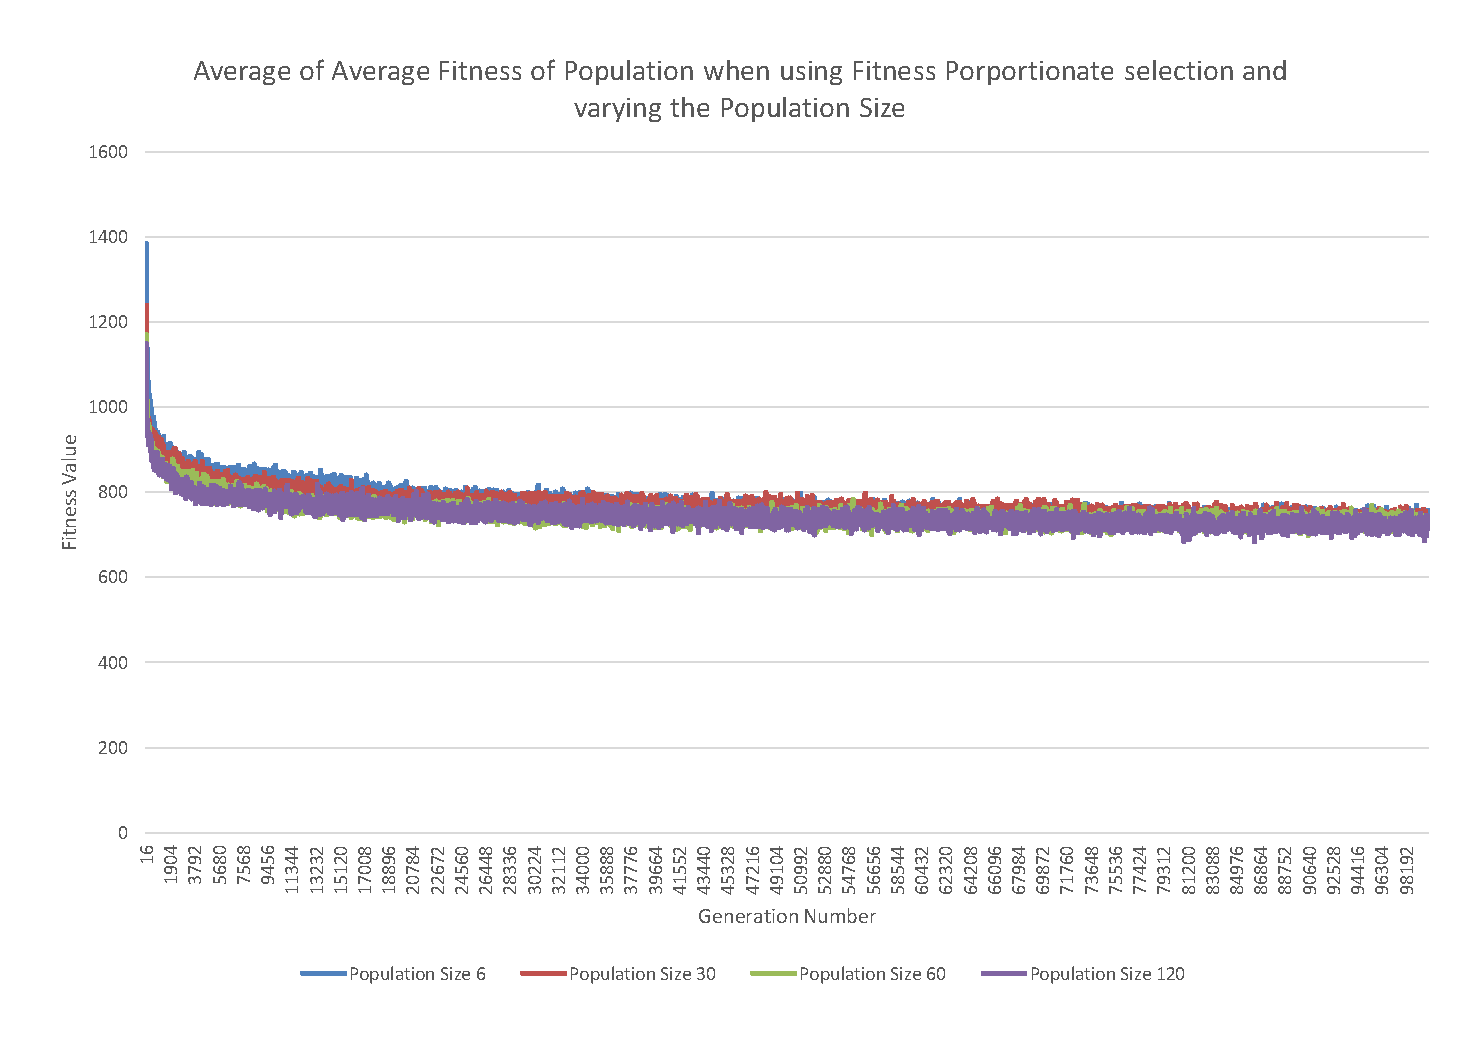
\includegraphics[height=0.945\textwidth]{figures/CircleTests/PopulationSizeControl/CirclePopulationSizeControllAverageAverage.pdf}}
	\caption{Population Size Control - Average Average}
\end{figure}
\end{landscape}

\begin{landscape}
\begin{figure}[thbp]
	\centerline{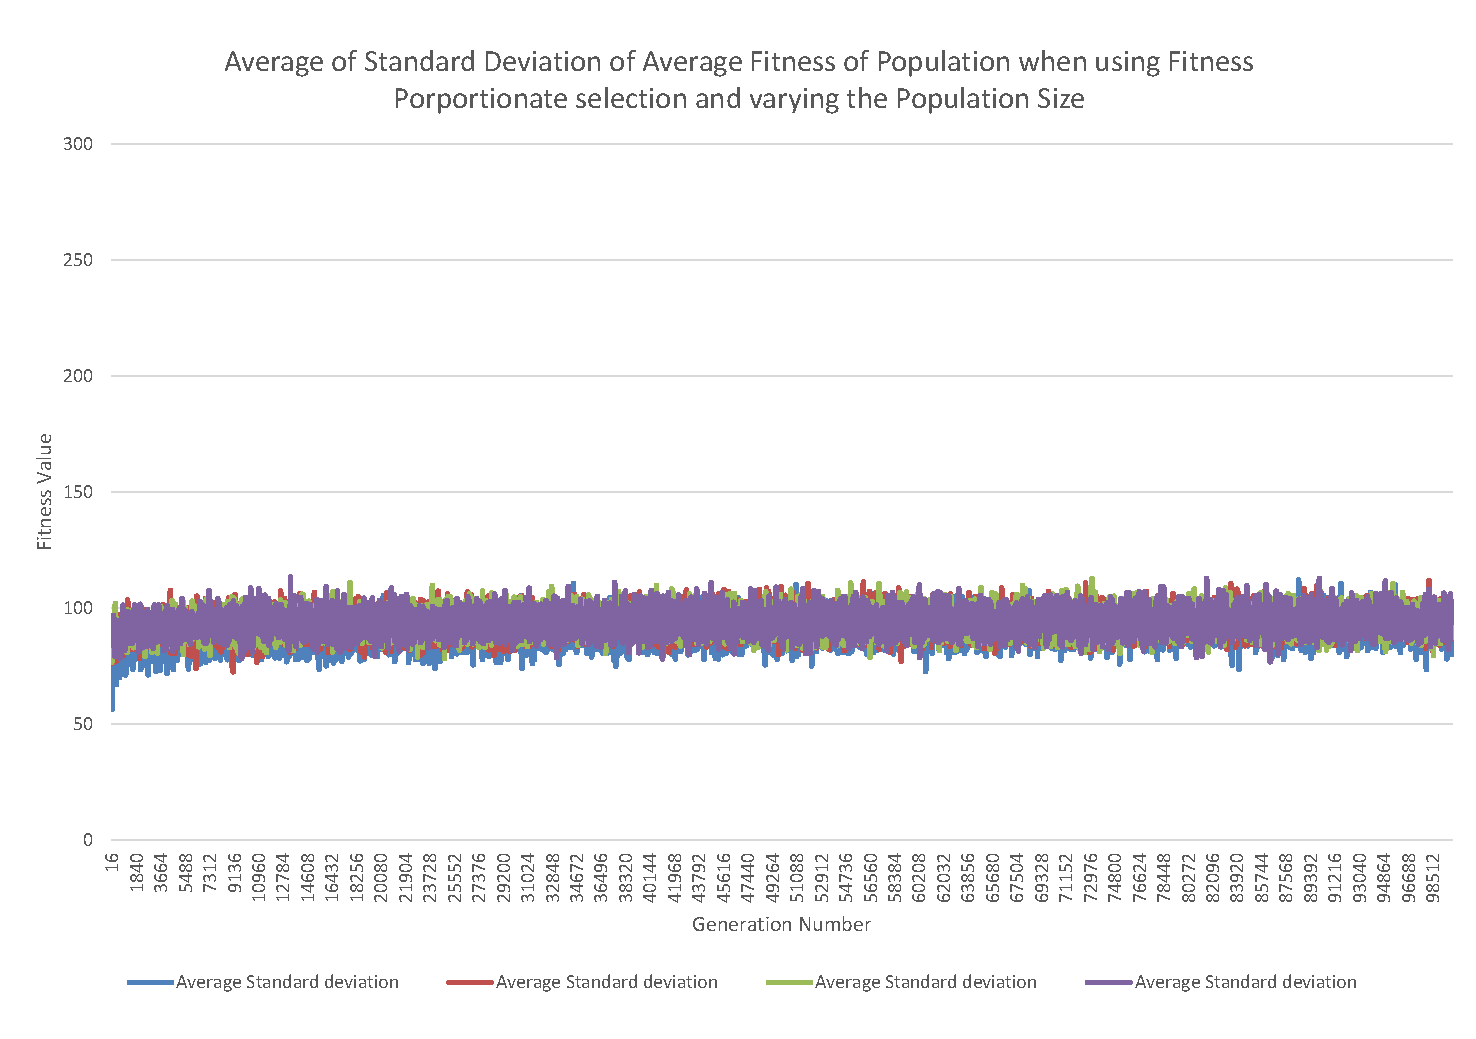
\includegraphics[height=0.945\textwidth]{figures/CircleTests/PopulationSizeControl/CirclePopulationSizeControllAverageStandardDeviation.pdf}}
	\caption{Population Size Control - Average Standard Deviation}
\end{figure}
\end{landscape}

% section population_size_control_results (end)

% chapter memetic_algorithm_tunin_results (end)






\chapter{BHW1 Benchmark Results} % (fold)
\label{cha:bhw1_benchmark_results}

\begin{landscape}
\begin{figure}[thbp]
	\centerline{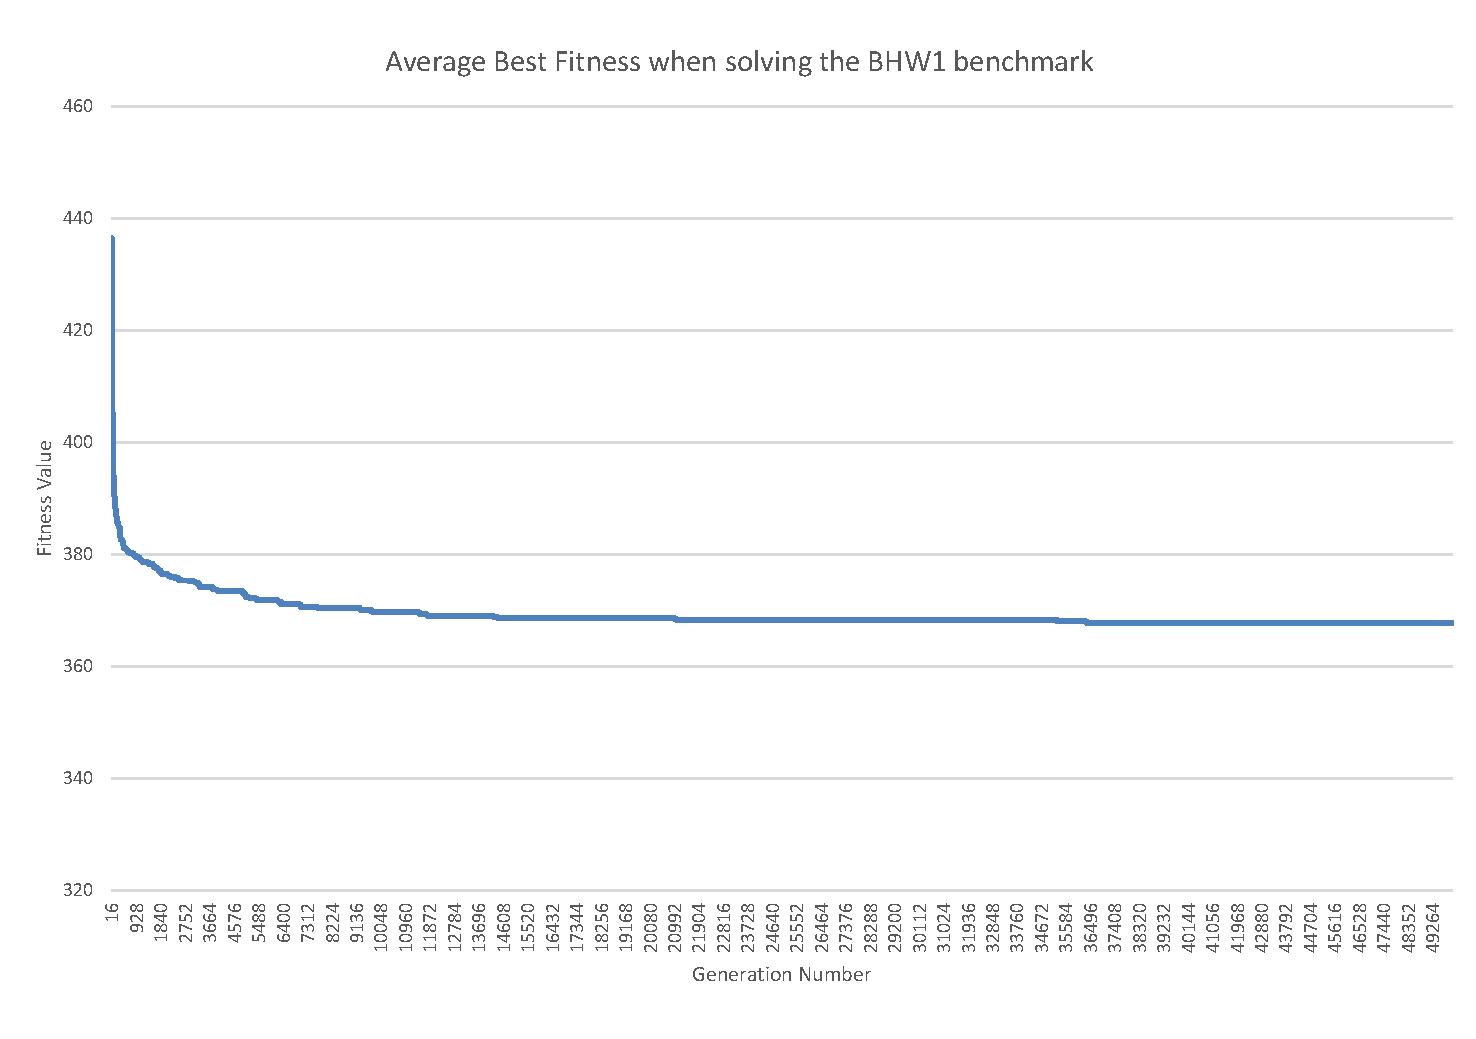
\includegraphics[height=0.945\textwidth]{figures/BHW1_graphs/BHW1_average_best.pdf}}
	\caption{BHW1 - Average Best}
	\label{fig:bhw1ab}
\end{figure}
\end{landscape}

\begin{landscape}
\begin{figure}[thbp]
	\centerline{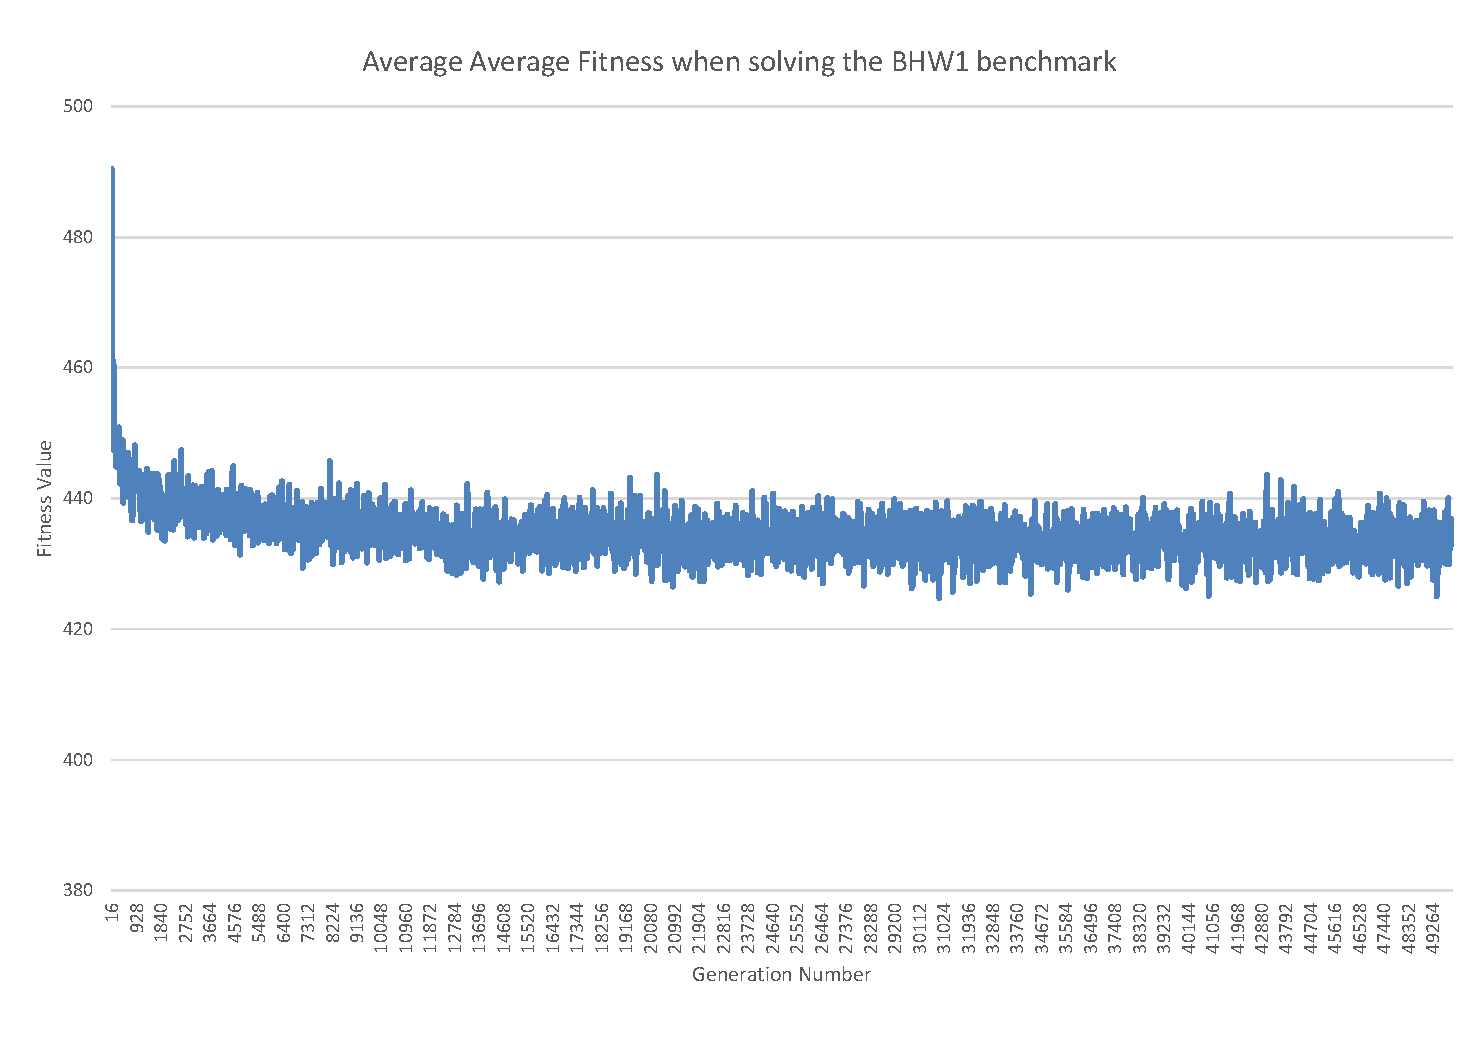
\includegraphics[height=0.945\textwidth]{figures/BHW1_graphs/BHW1_average_average.pdf}}
	\caption{Population Size Control - Average Average}
	\label{fig:bhw1aa}
\end{figure}
\end{landscape}

\begin{landscape}
\begin{figure}[thbp]
	\centerline{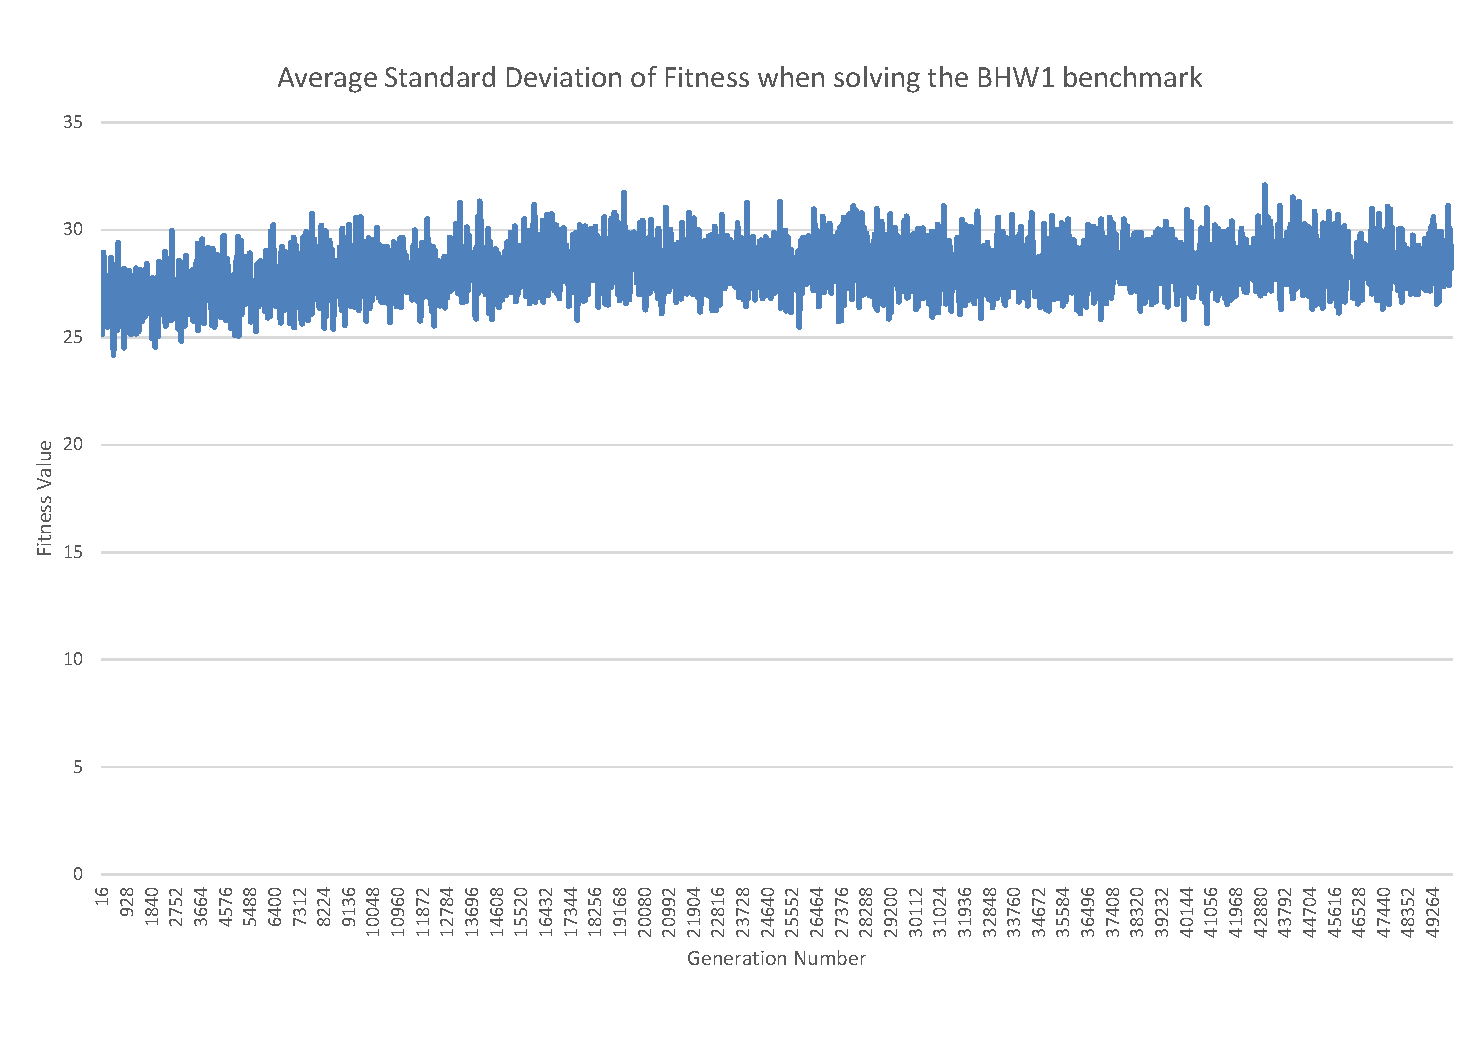
\includegraphics[height=0.945\textwidth]{figures/BHW1_graphs/BHW1_average_standard_deviation.pdf}}
	\caption{BHW1 - Average Standard Deviation}
	\label{fig:bhw1astd}
\end{figure}
\end{landscape}

% chapter bhw1_benchmark_results (end)



\chapter{How Routes are Driven as Drawn by the Drivers} % (fold)
\label{cha:how_routes_are_driven_as_drawn_by_the_drivers}

\includepdf[landscape=true,pages={-},pagecommand={\pagestyle{fancy}},height=\textwidth]{figures/Routes/DrivenDrawn/Broeteruter_slik_de_blir_kjoert-nummerert.pdf}

% chapter how_routes_are_driven_as_drawn_by_the_drivers (end)




\chapter{Graphs of the Performance of the MA when Applied to Map Data from Trondheim} % (fold)
\label{cha:gotpotmwatmdft}

\section{Route 310174\_KV\_B\_Midtbyen} % (fold)
\label{sec:route_310174_KV_B_Midtbyen}

\subsection{Graphs of Performance when Run for 100000 Generations} % (fold)
\label{sub:graphs_of_performance_when_run_for_100000_generations_KV_B}

\begin{landscape}
\begin{figure}[thbp]
	\centerline{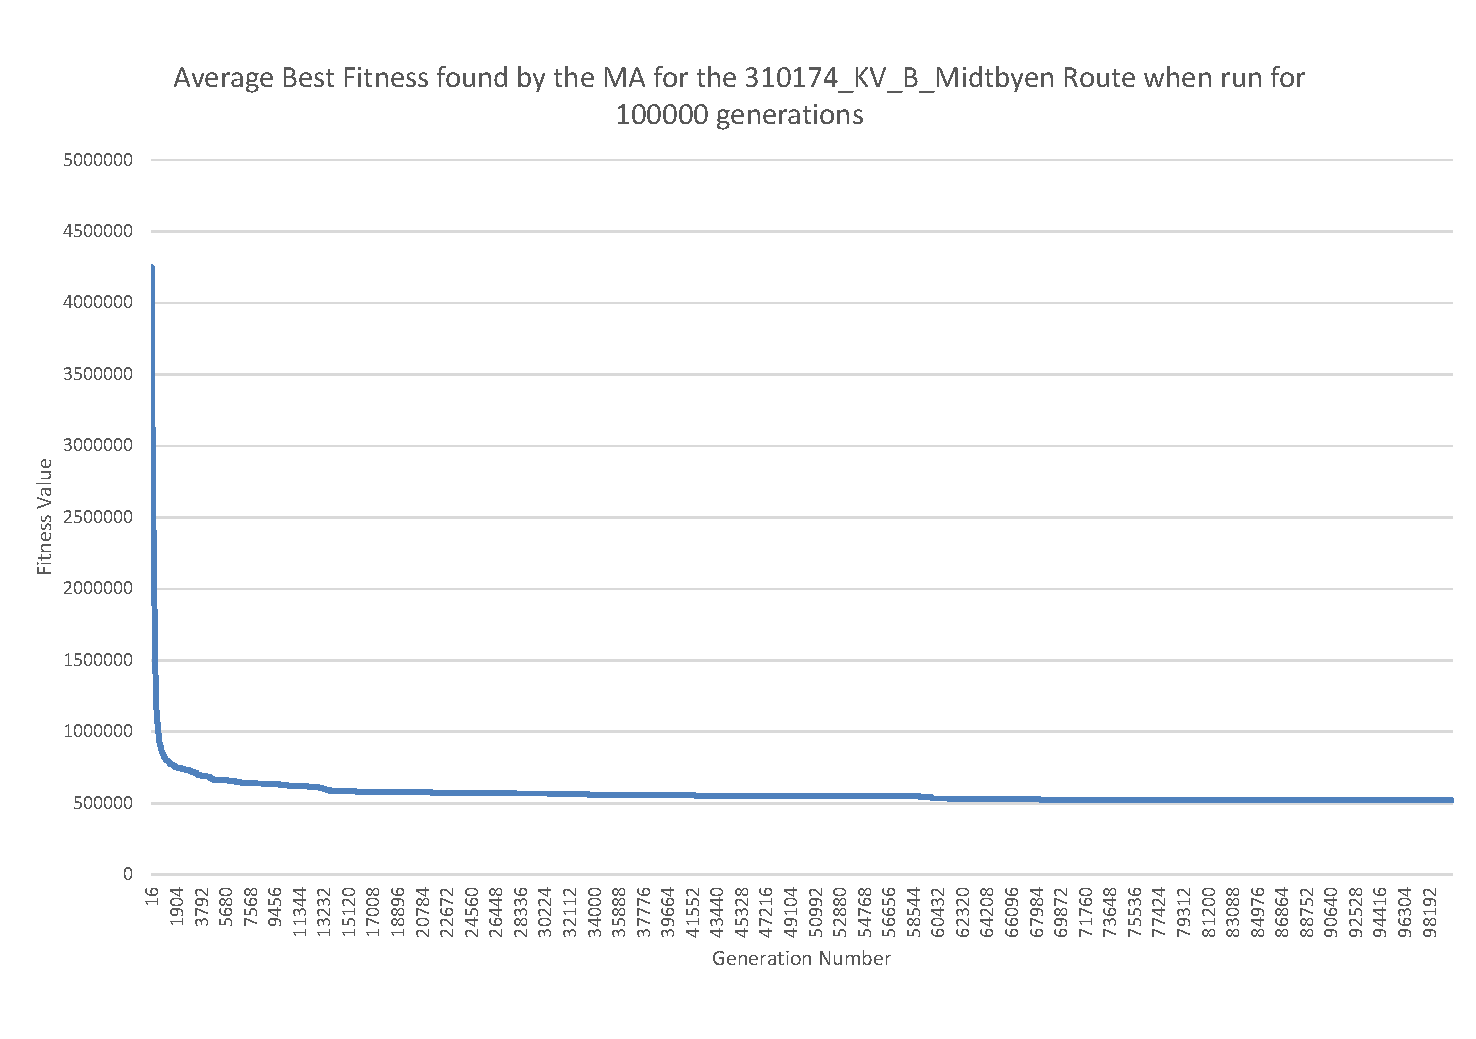
\includegraphics[height=0.945\textwidth]{figures/Trondheim_graphs/KV_B/KV_B-100k_average_best.pdf}}
	\caption{Route 310174\_KV\_B\_Midtbyen 100000 Generations - Average Best}
	\label{fig:KV_B_100k_ab}
\end{figure}
\end{landscape}

\begin{landscape}
\begin{figure}[thbp]
	\centerline{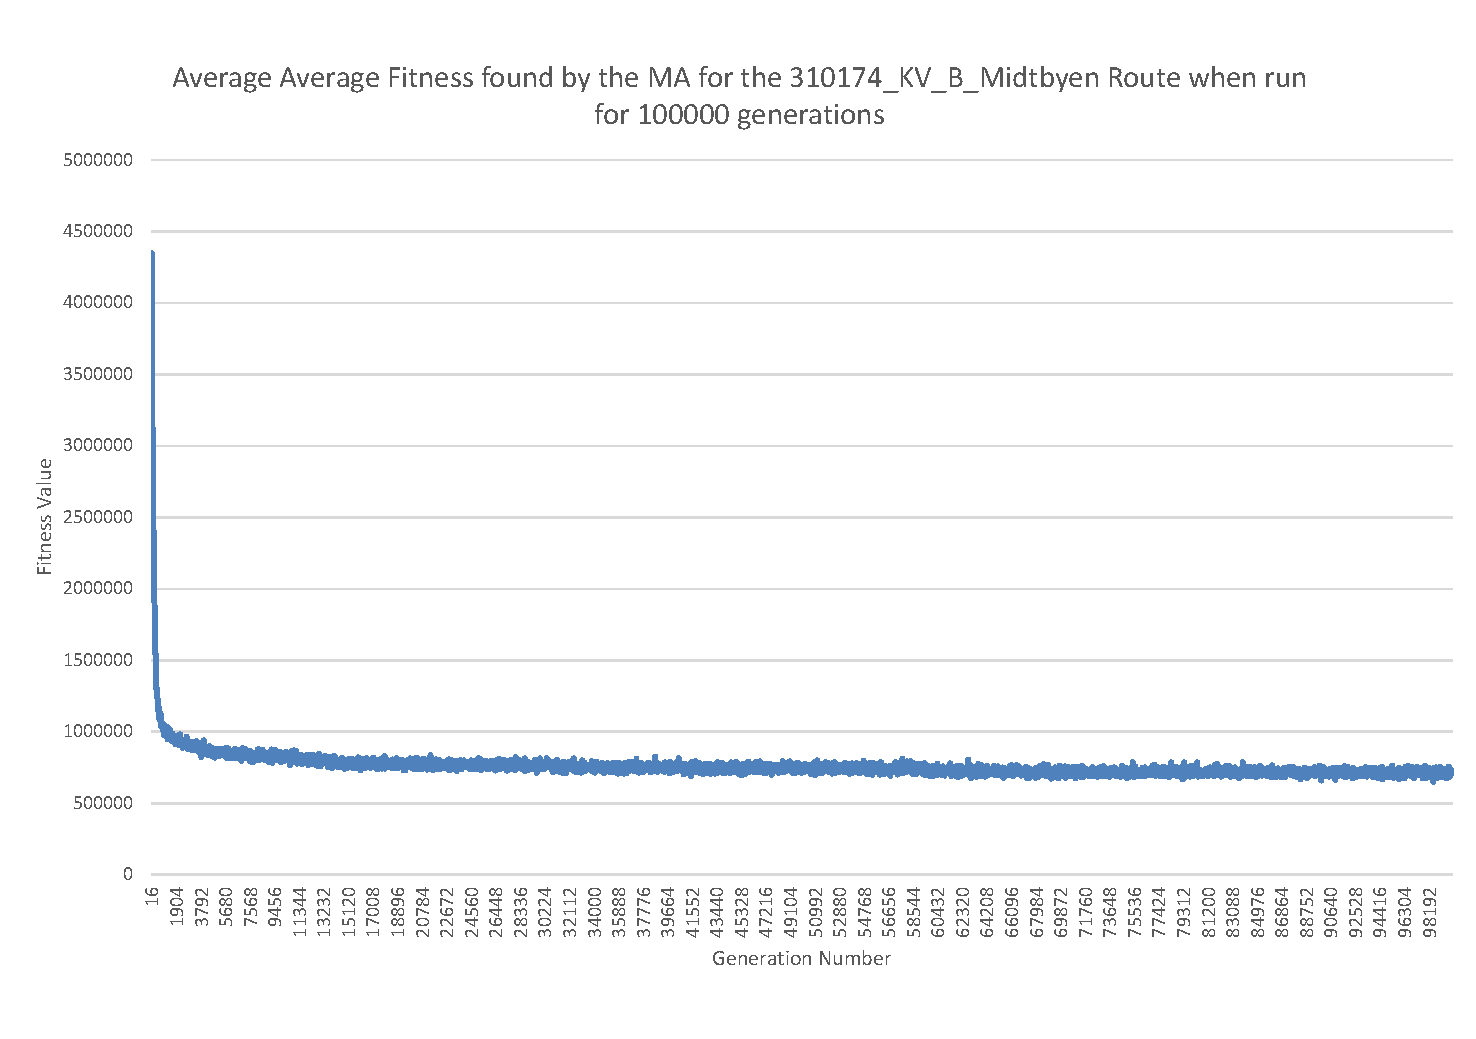
\includegraphics[height=0.945\textwidth]{figures/Trondheim_graphs/KV_B/KV_B-100k_average_average.pdf}}
	\caption{Route 310174\_KV\_B\_Midtbyen 100000 Generations - Average Average}
	\label{fig:KV_B_100k_aa}
\end{figure}
\end{landscape}

\begin{landscape}
\begin{figure}[thbp]
	\centerline{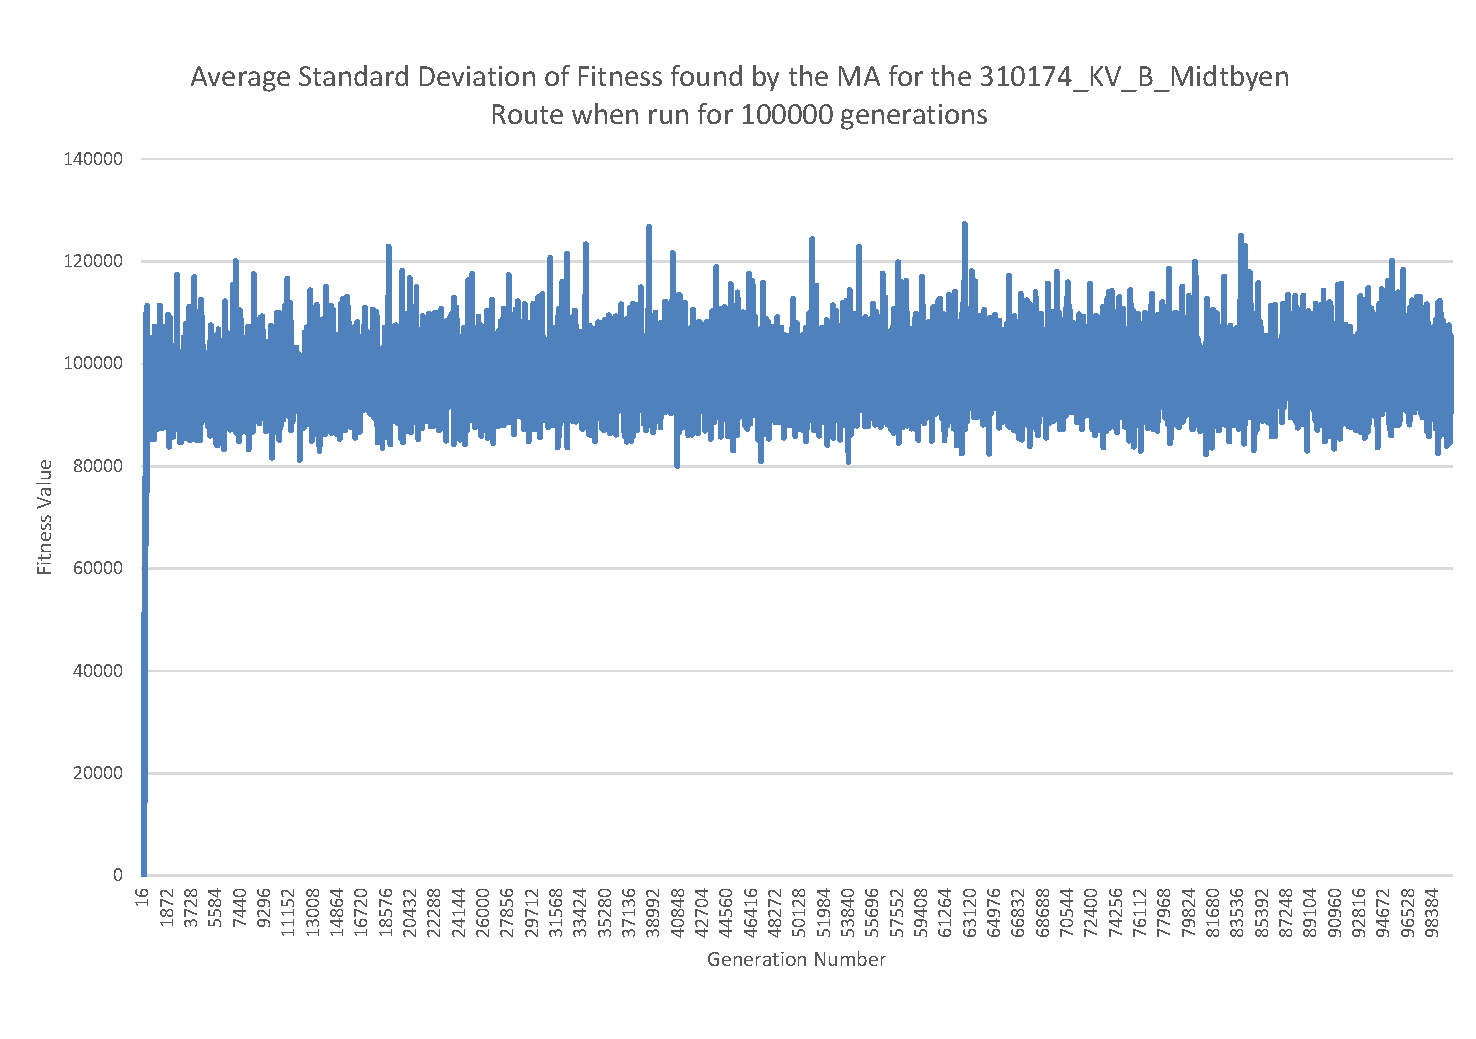
\includegraphics[height=0.945\textwidth]{figures/Trondheim_graphs/KV_B/KV_B-100k_average_standard_deviation.pdf}}
	\caption{Route 310174\_KV\_B\_Midtbyen 100000 Generations - Average Standard Deviation}
	\label{fig:KV_B_100k_astd}
\end{figure}
\end{landscape}

% subsection graphs_of_performance_when_run_for_100000_generations (end)



\subsection{Graphs of Performance when Run for 50000 Generations} % (fold)
\label{sub:graphs_of_performance_when_run_for_50000_generations_KV_B}

\begin{landscape}
\begin{figure}[thbp]
	\centerline{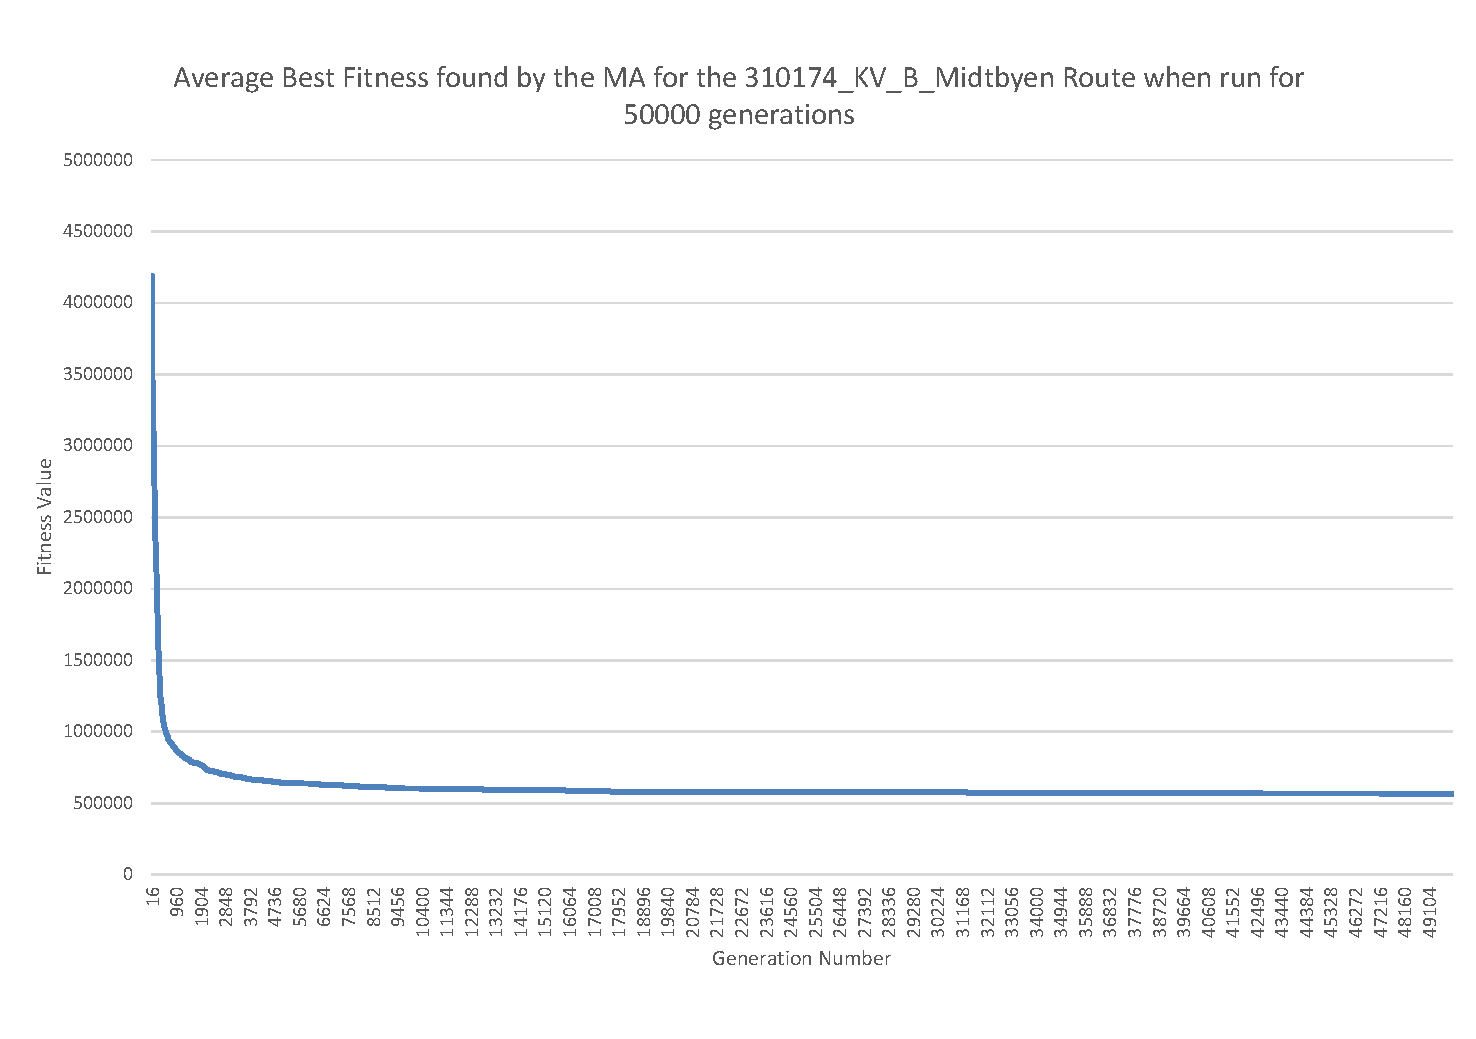
\includegraphics[height=0.945\textwidth]{figures/Trondheim_graphs/KV_B/KV_B-all_average_best.pdf}}
	\caption{Route 310174\_KV\_B\_Midtbyen 50000 Generations - Average Best}
	\label{fig:KV_B_50k_ab}
\end{figure}
\end{landscape}

\begin{landscape}
\begin{figure}[thbp]
	\centerline{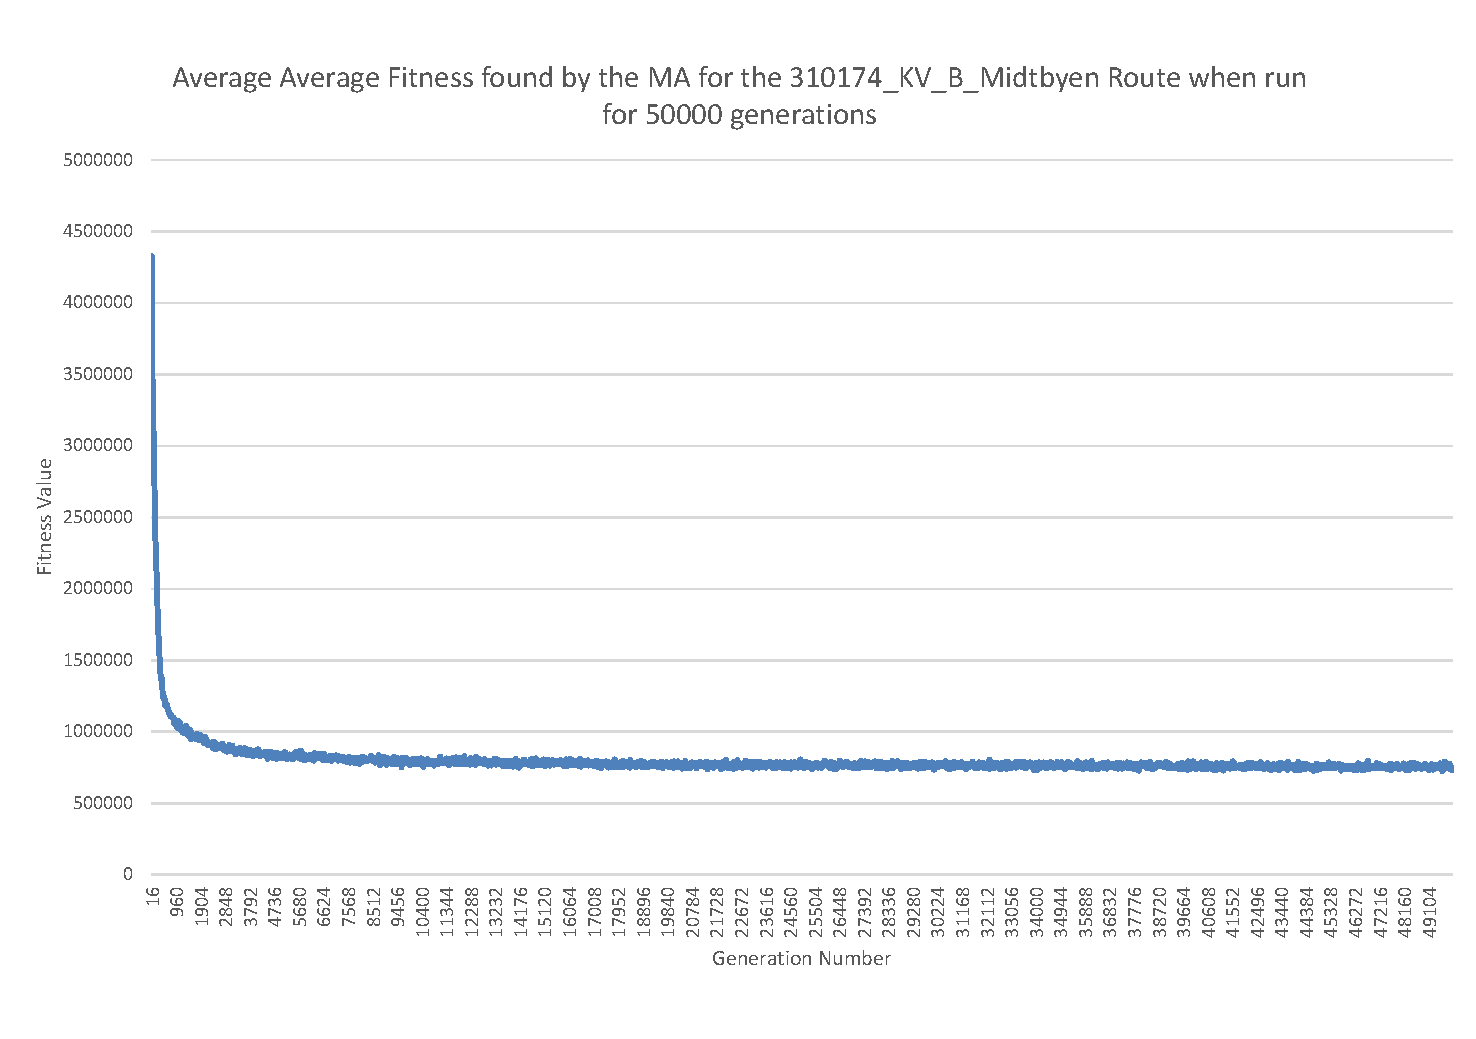
\includegraphics[height=0.945\textwidth]{figures/Trondheim_graphs/KV_B/KV_B-all_average_average.pdf}}
	\caption{Route 310174\_KV\_B\_Midtbyen 50000 Generations - Average Average}
	\label{fig:KV_B_50k_aa}
\end{figure}
\end{landscape}

\begin{landscape}
\begin{figure}[thbp]
	\centerline{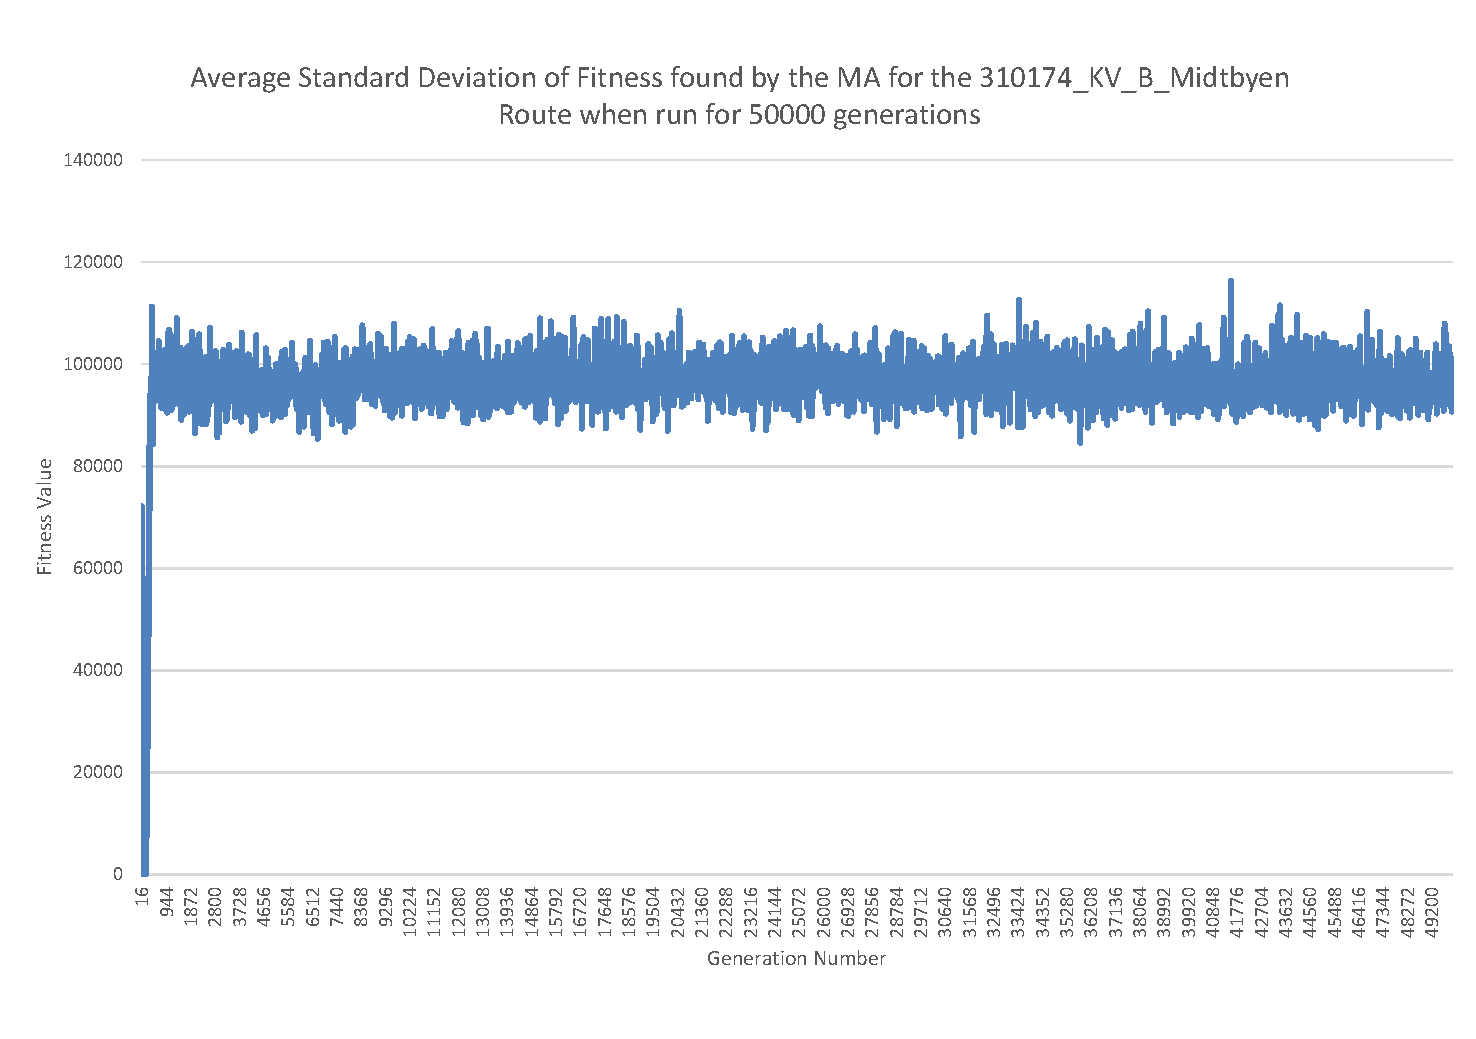
\includegraphics[height=0.945\textwidth]{figures/Trondheim_graphs/KV_B/KV_B-all_average_standard_deviation.pdf}}
	\caption{Route 310174\_KV\_B\_Midtbyen 50000 Generations - Average Standard Deviation}
	\label{fig:KV_B_50k_astd}
\end{figure}
\end{landscape}

% subsection graphs_of_performance_when_run_for_50000_generations (end)

% section route_310174_ (end)




\section{Route 310179\_KV\_H\_Midtbyen} % (fold)
\label{sec:route_310179_kv_h_midtbyen}

\subsection{Graphs of Performance when Run for 100000 Generations} % (fold)
\label{sub:graphs_of_performance_when_run_for_100000_generations_KV_H}

\begin{landscape}
\begin{figure}[thbp]
	\centerline{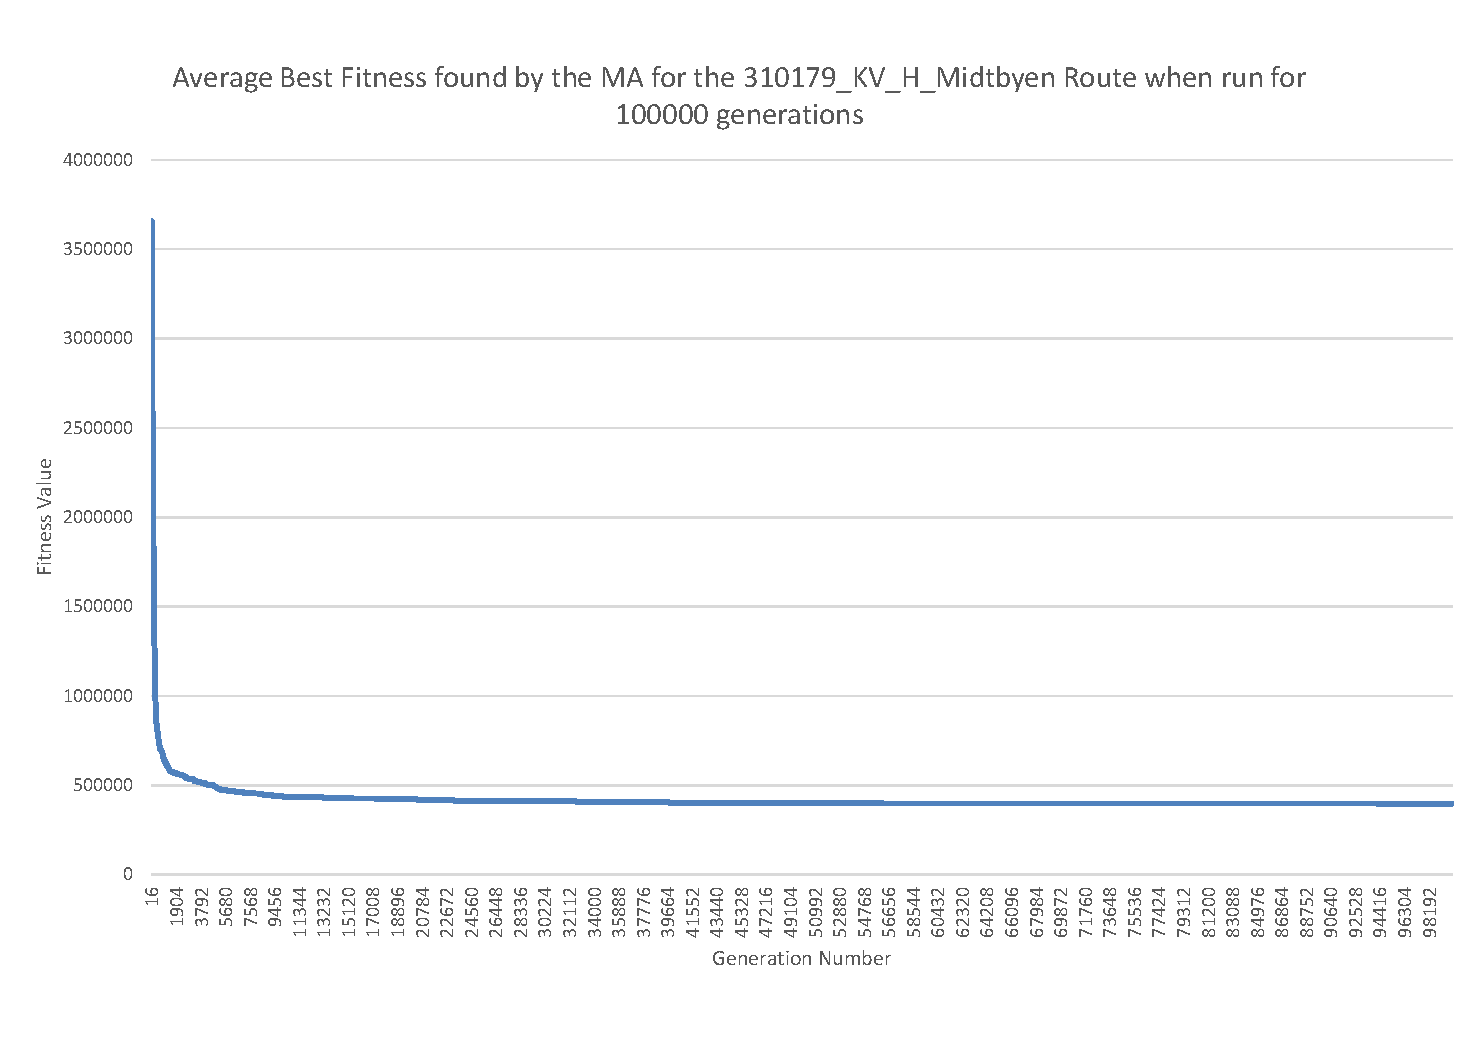
\includegraphics[height=0.945\textwidth]{figures/Trondheim_graphs/KV_H/KV_H-100k_average_best.pdf}}
	\caption{Route 310179\_KV\_H\_Midtbyen 100000 Generations - Average Best}
	\label{fig:KV_H_100k_ab}
\end{figure}
\end{landscape}

\begin{landscape}
\begin{figure}[thbp]
	\centerline{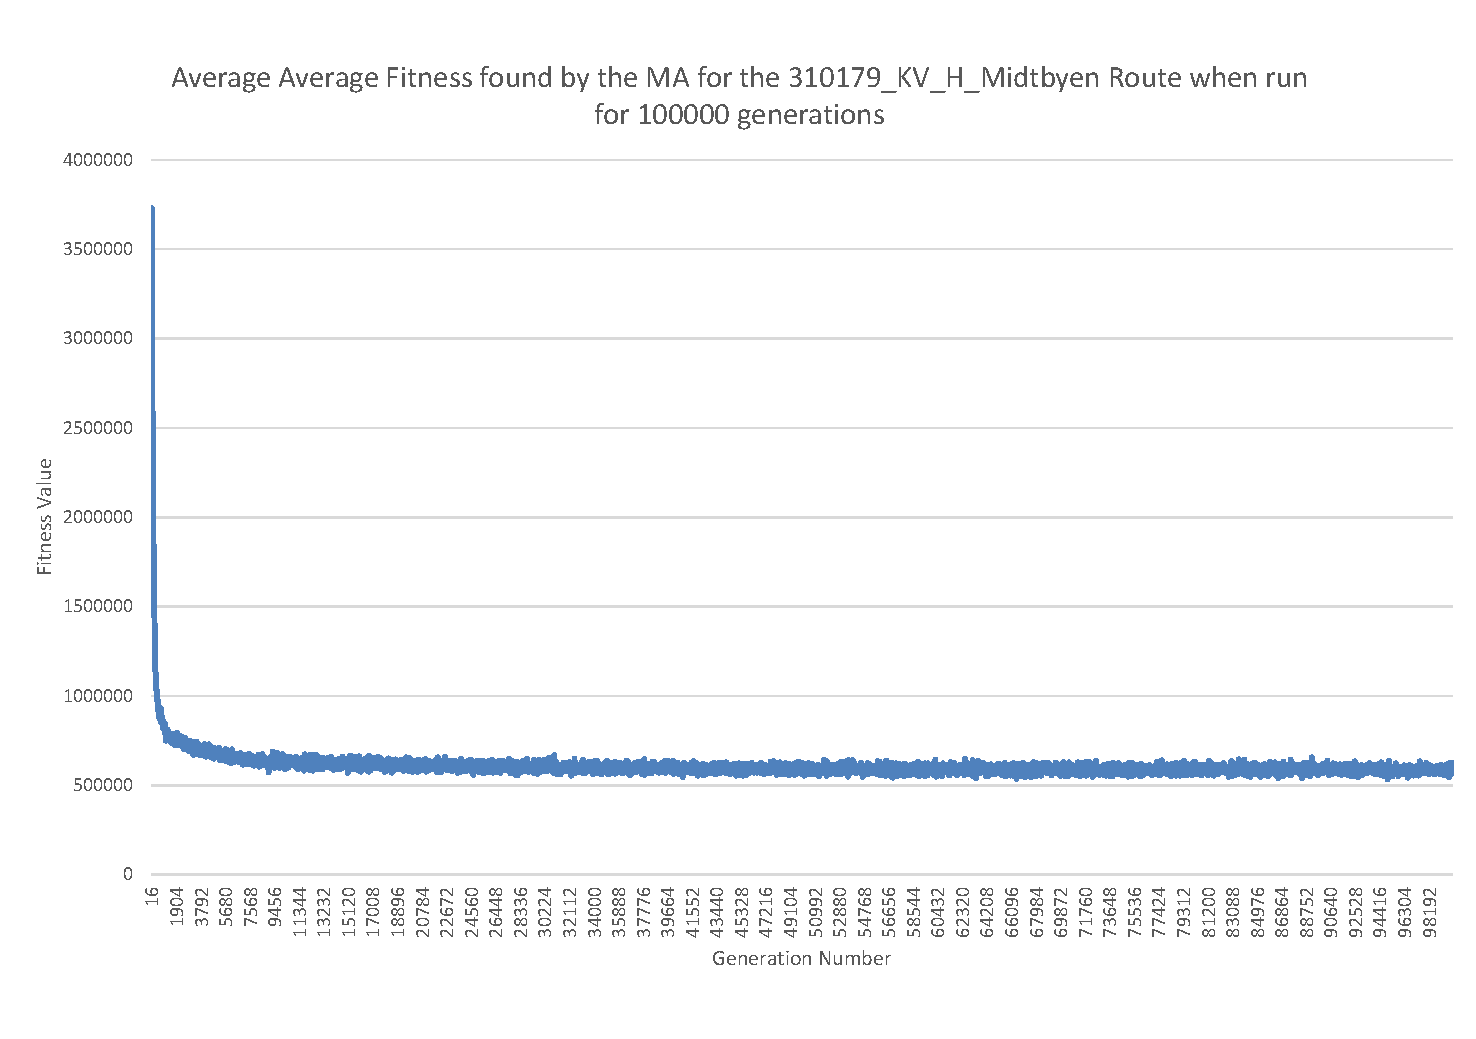
\includegraphics[height=0.945\textwidth]{figures/Trondheim_graphs/KV_H/KV_H-100k_average_average.pdf}}
	\caption{Route 310179\_KV\_H\_Midtbyen 100000 Generations - Average Average}
	\label{fig:KV_H_100k_aa}
\end{figure}
\end{landscape}

\begin{landscape}
\begin{figure}[thbp]
	\centerline{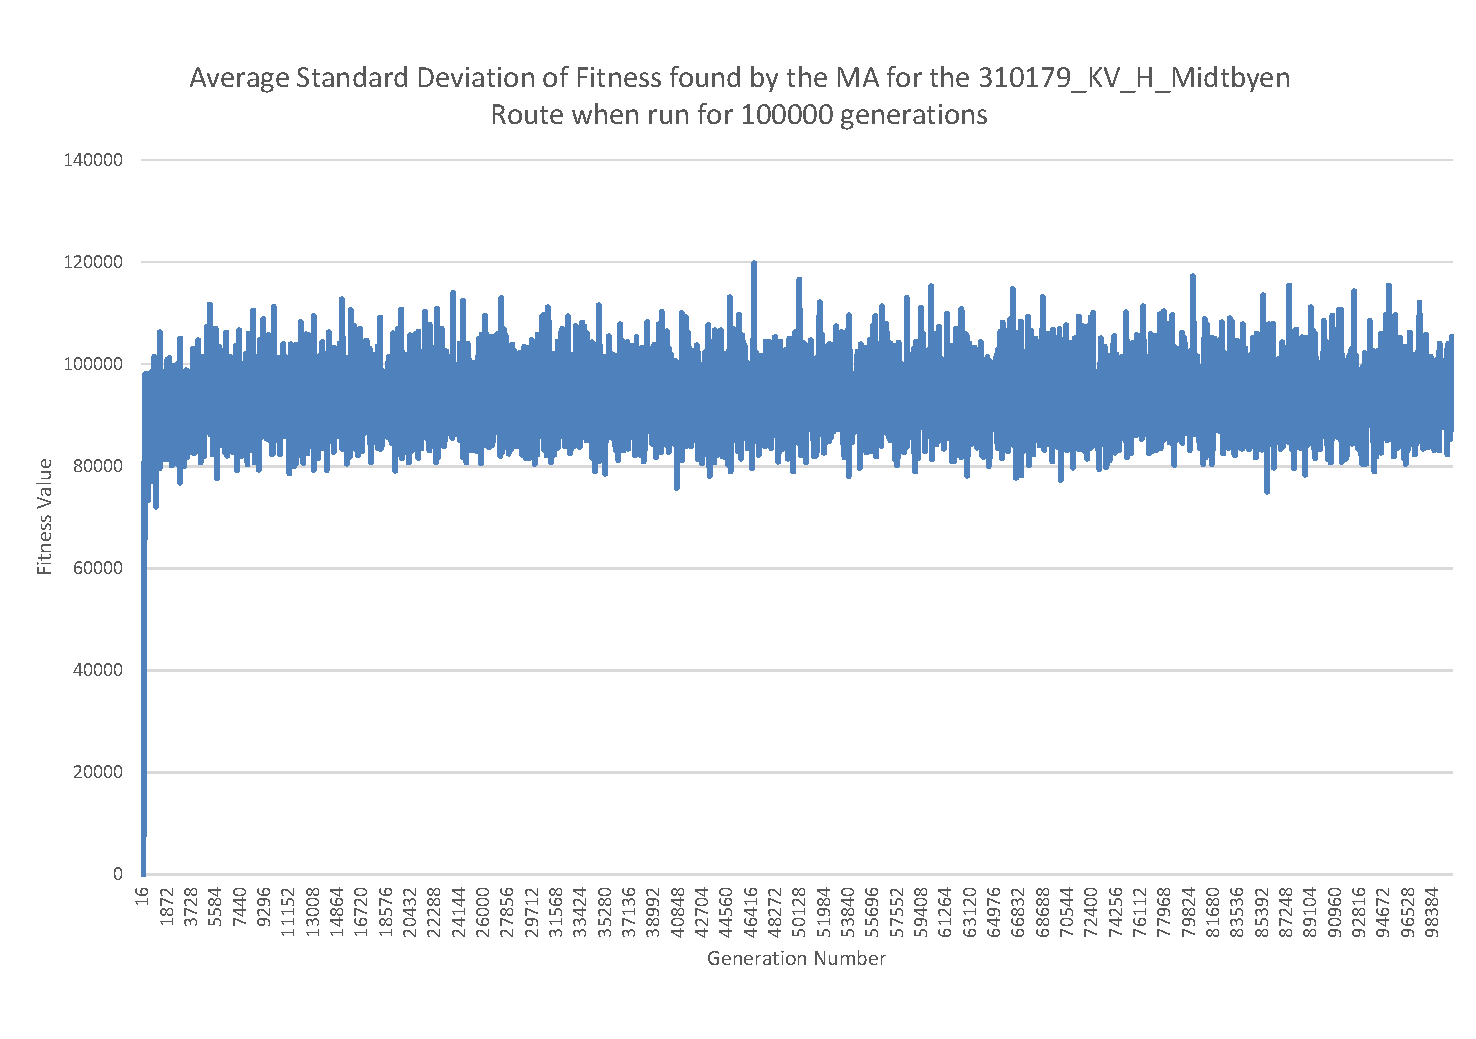
\includegraphics[height=0.945\textwidth]{figures/Trondheim_graphs/KV_H/KV_H-100k_average_standard_deviation.pdf}}
	\caption{Route 310179\_KV\_H\_Midtbyen 100000 Generations - Average Standard Deviation}
	\label{fig:KV_H_100k_astd}
\end{figure}
\end{landscape}

% subsection graphs_of_performance_when_run_for_100000_generations (end)




\subsection{Graphs of Performance when Run for 50000 Generations} % (fold)
\label{sub:graphs_of_performance_when_run_for_50000_generations_KV_H}

\begin{landscape}
\begin{figure}[thbp]
	\centerline{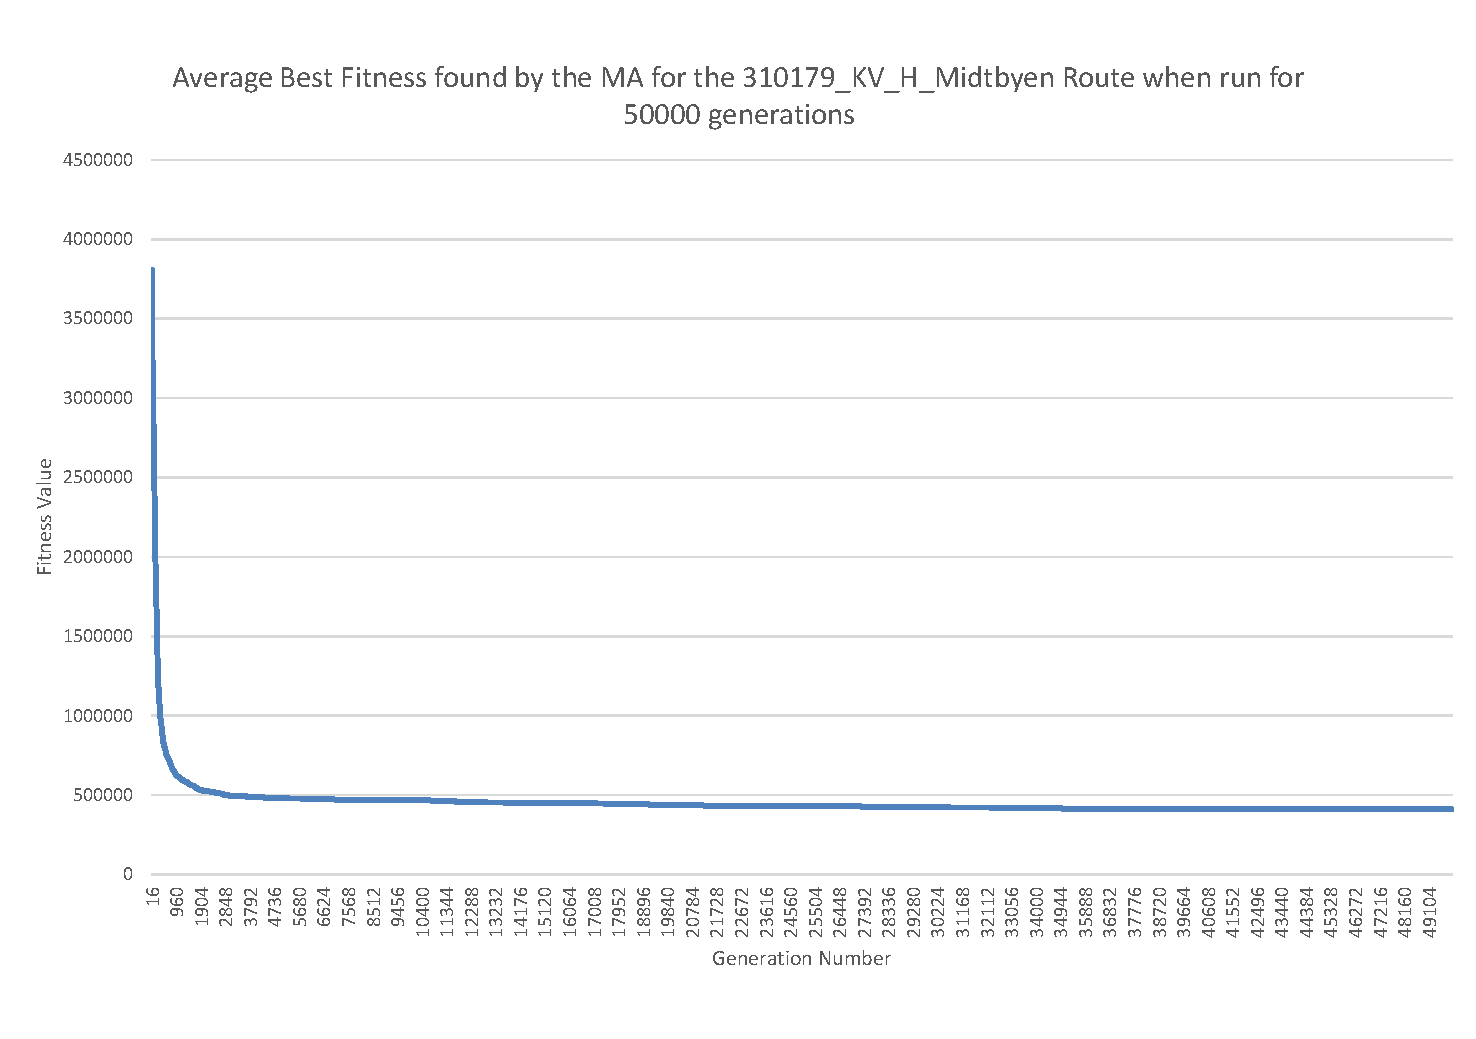
\includegraphics[height=0.945\textwidth]{figures/Trondheim_graphs/KV_H/KV_H-all_average_best.pdf}}
	\caption{Route 310179\_KV\_B\_Midtbyen 50000 Generations - Average Best}
	\label{fig:KV_H_50k_ab}
\end{figure}
\end{landscape}

\begin{landscape}
\begin{figure}[thbp]
	\centerline{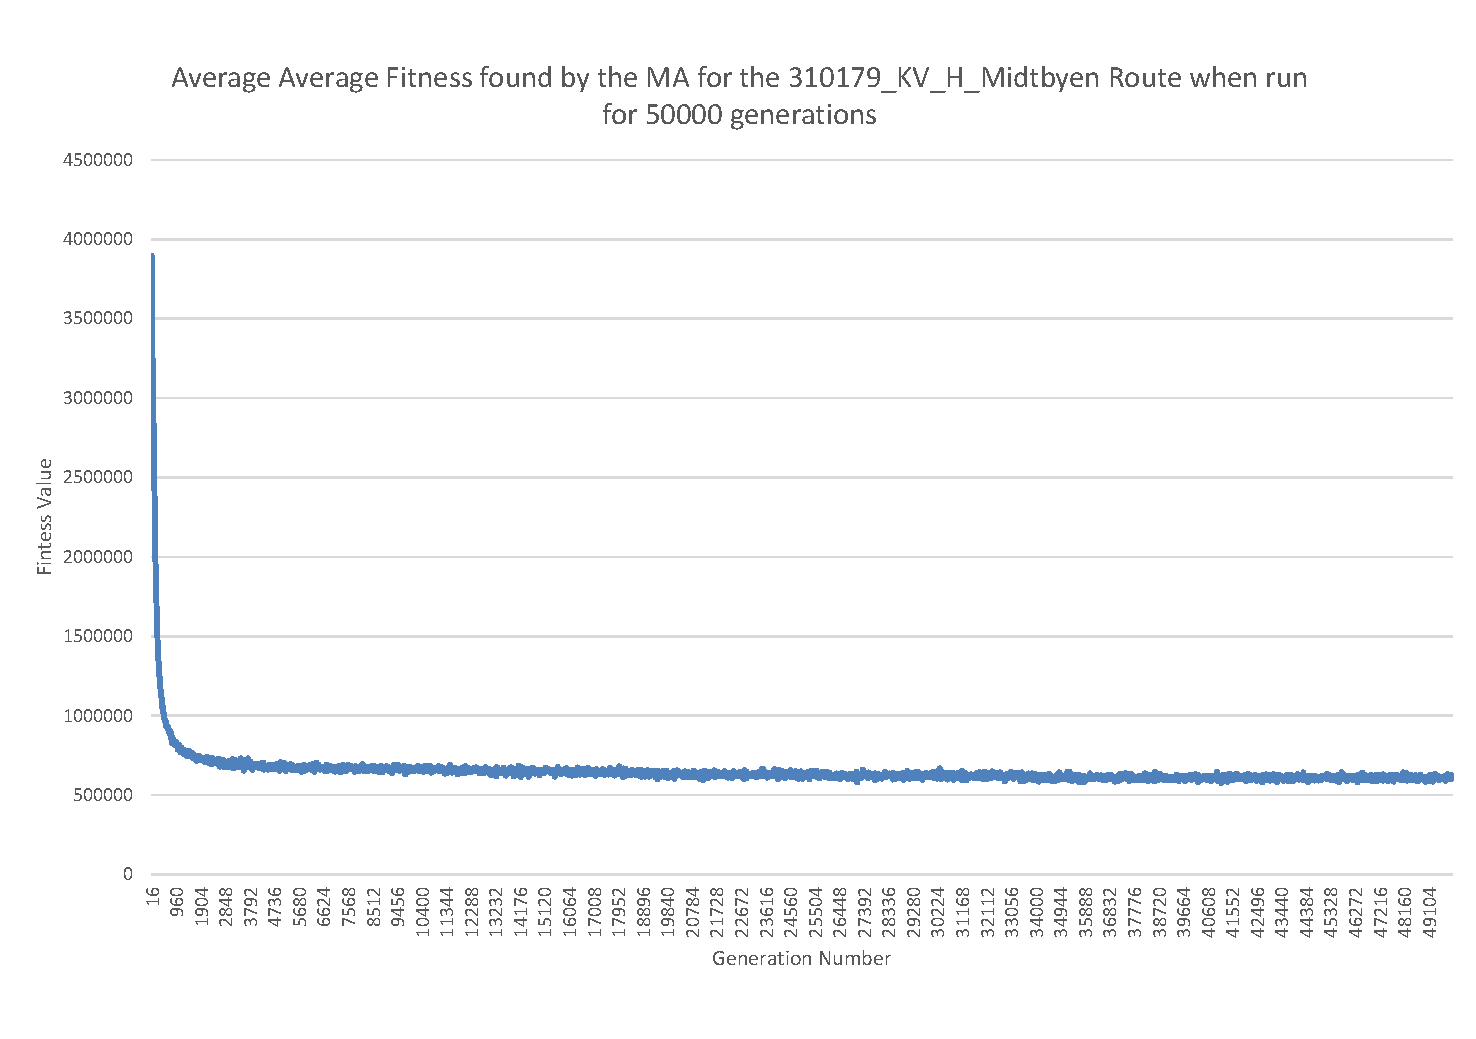
\includegraphics[height=0.945\textwidth]{figures/Trondheim_graphs/KV_H/KV_H-all_average_average.pdf}}
	\caption{Route 310179\_KV\_B\_Midtbyen 50000 Generations - Average Average}
	\label{fig:KV_H_50k_aa}
\end{figure}
\end{landscape}

\begin{landscape}
\begin{figure}[thbp]
	\centerline{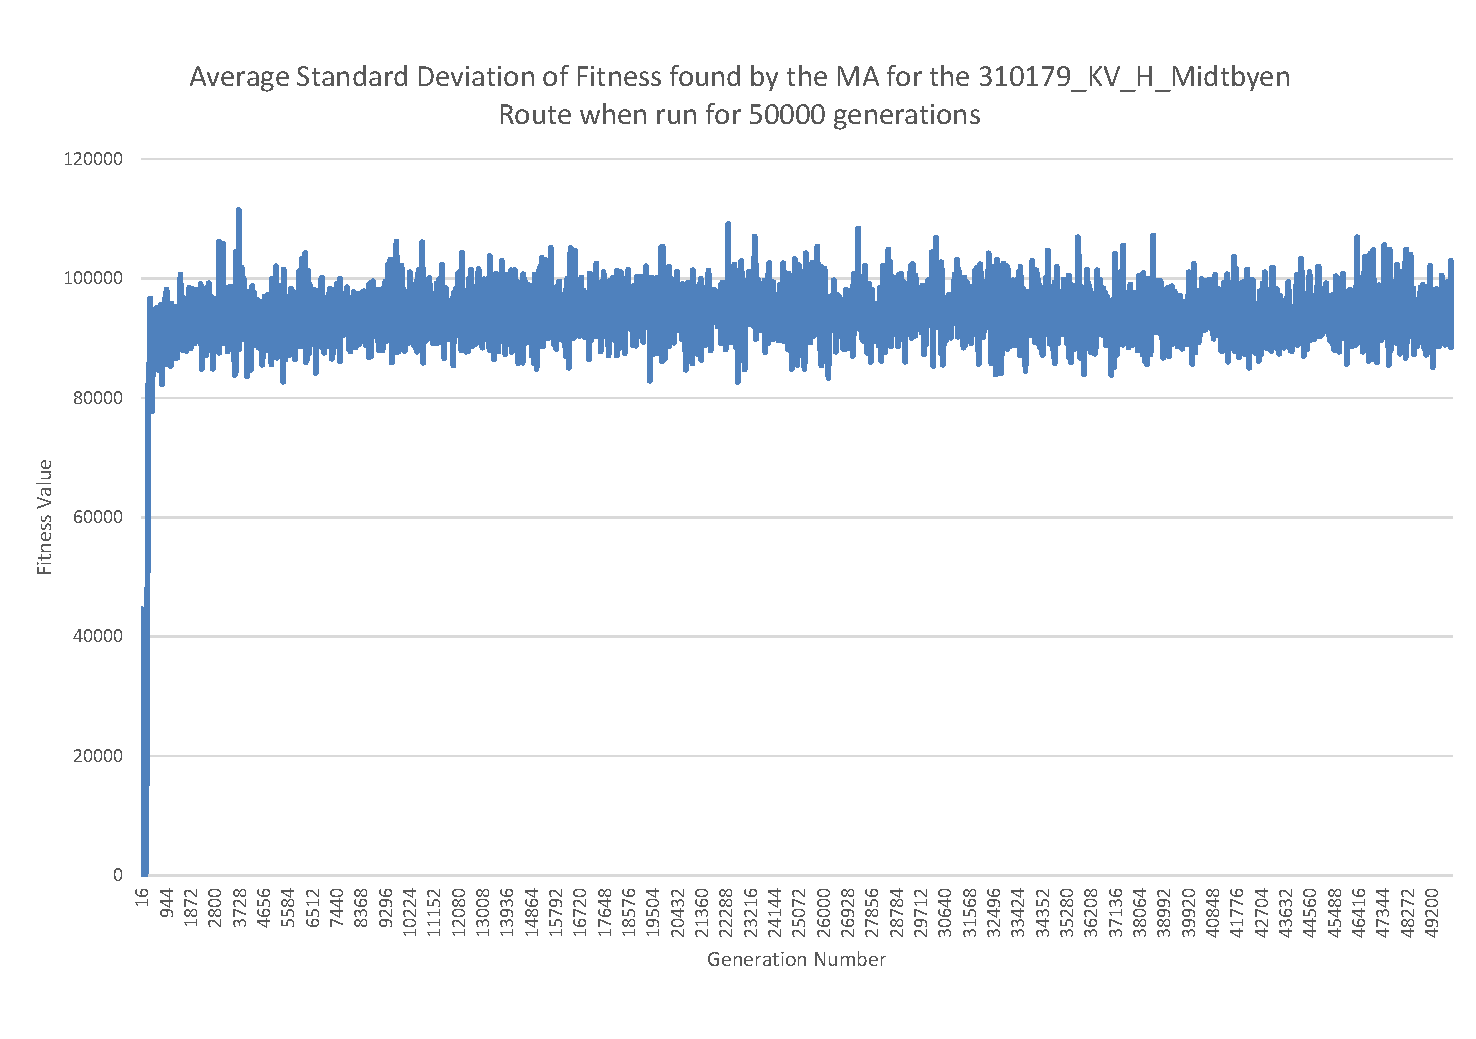
\includegraphics[height=0.945\textwidth]{figures/Trondheim_graphs/KV_H/KV_H-all_average_standard_deviation.pdf}}
	\caption{Route 310179\_KV\_B\_Midtbyen 50000 Generations - Average Standard Deviation}
	\label{fig:KV_H_50k_astd}
\end{figure}
\end{landscape}

% subsection graphs_of_performance_when_run_for_50000_generations (end)

% section route_310179_kv_h_midtbyen (end)

% chapter gotpotmwatmdft (end)








\chapter{Pre-Project: Route Optimization for Winter Road Maintenance} % (fold)
\label{cha:pre_project_route_optimization_for_winter_road_maintenance}


\includepdf[pages={1-19},pagecommand={\pagestyle{fancy}},width=\textwidth]{Pre-Project_2014-Magnus_Thrap-Simon_Randby.pdf}

% chapter pre_project_route_optimization_for_winter_road_maintenance (end)












\chapter{Detailed Maps for the Generated Routes} % (fold)
\label{cha:detailed_maps_for_the_generated_routes}

\section{Detailed Generated Map for Route 310174\_KV\_B} % (fold)
\label{sec:detailed_generated_map_for_route_310174_kv_b}

% \begin{landscape}
% \begin{figure}[thbp]
	% \centerline{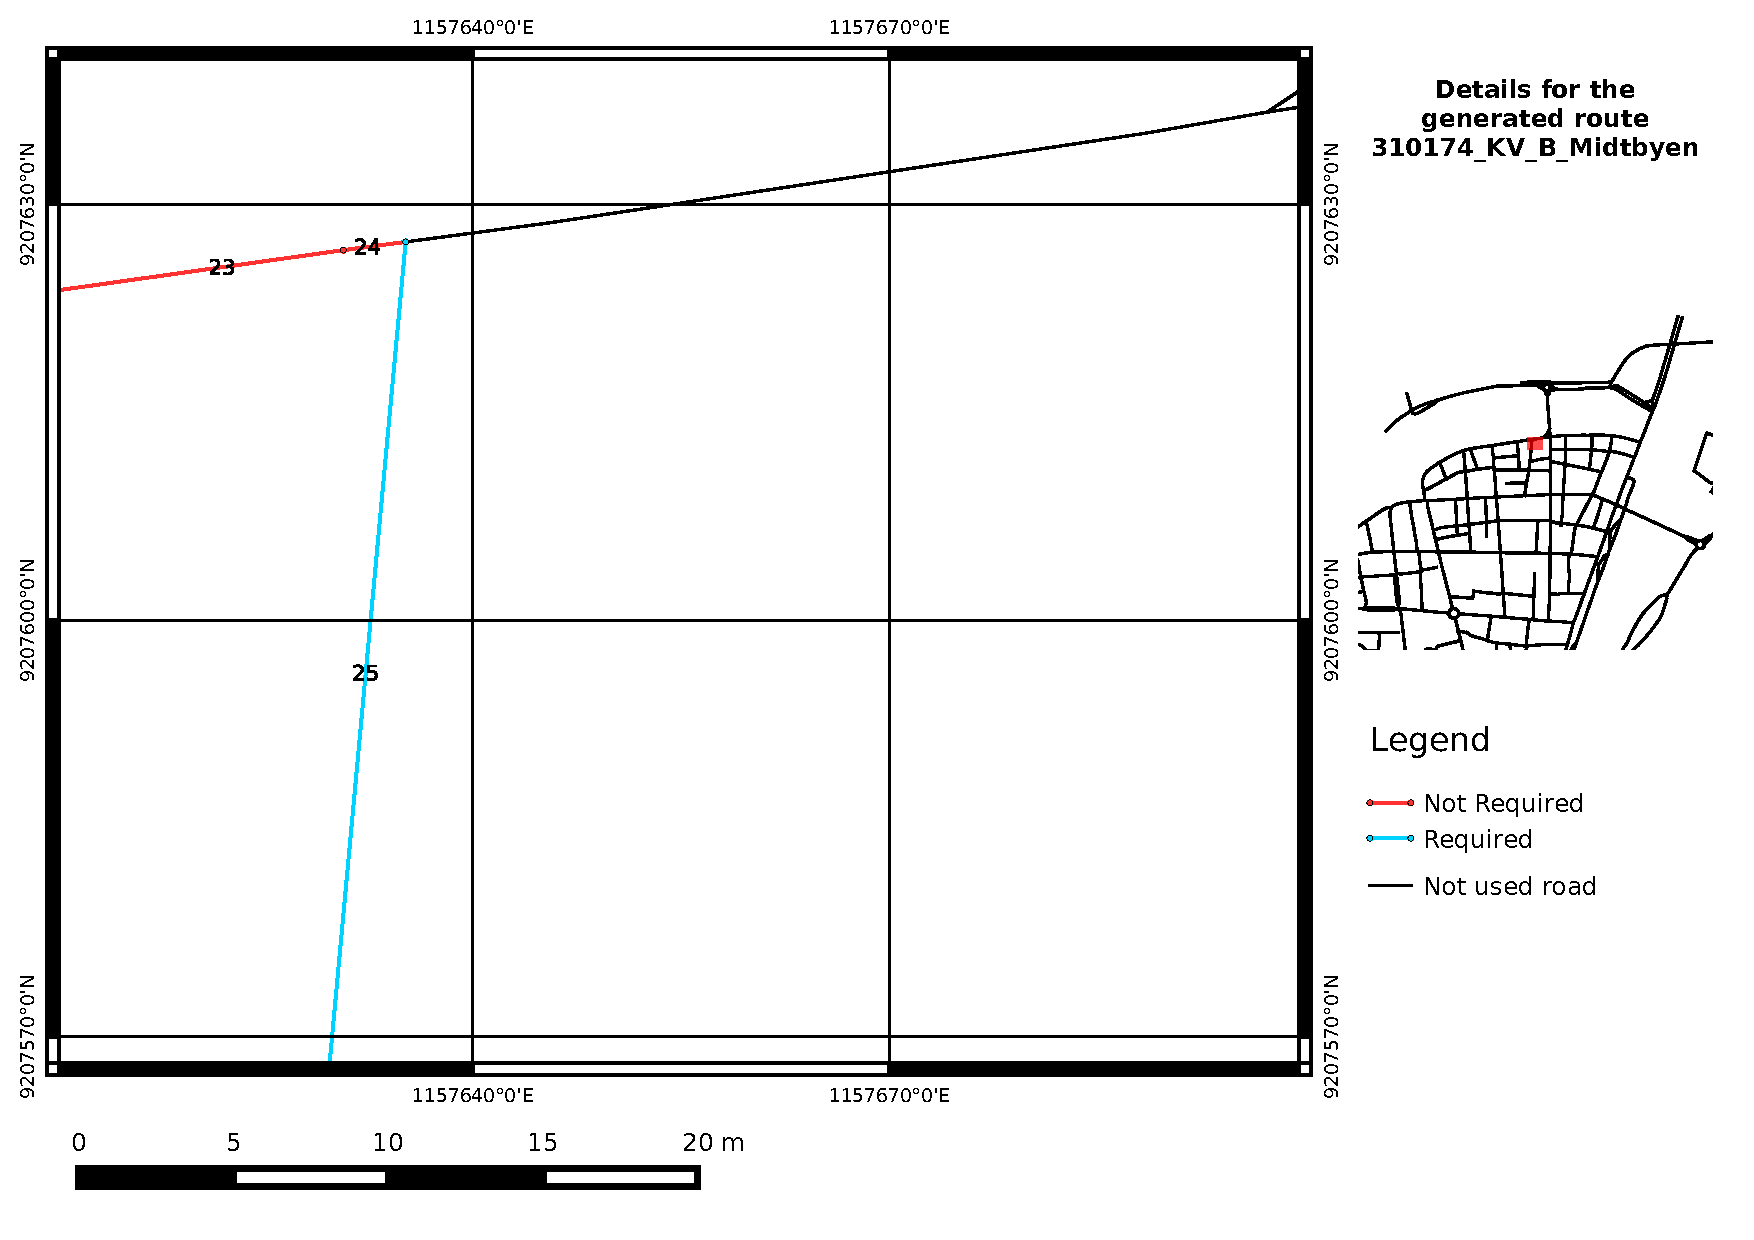
\includegraphics[height=0.945\textwidth]{figures/Routes/DetailedMaps-atlases/2015-06-23-final_detailed_atlas_for_KV_B_midtbyen.pdf}}
	% \caption{Mutation - Average Standard Deviation}
	% \label{fig:ctmasd}
% \end{figure}
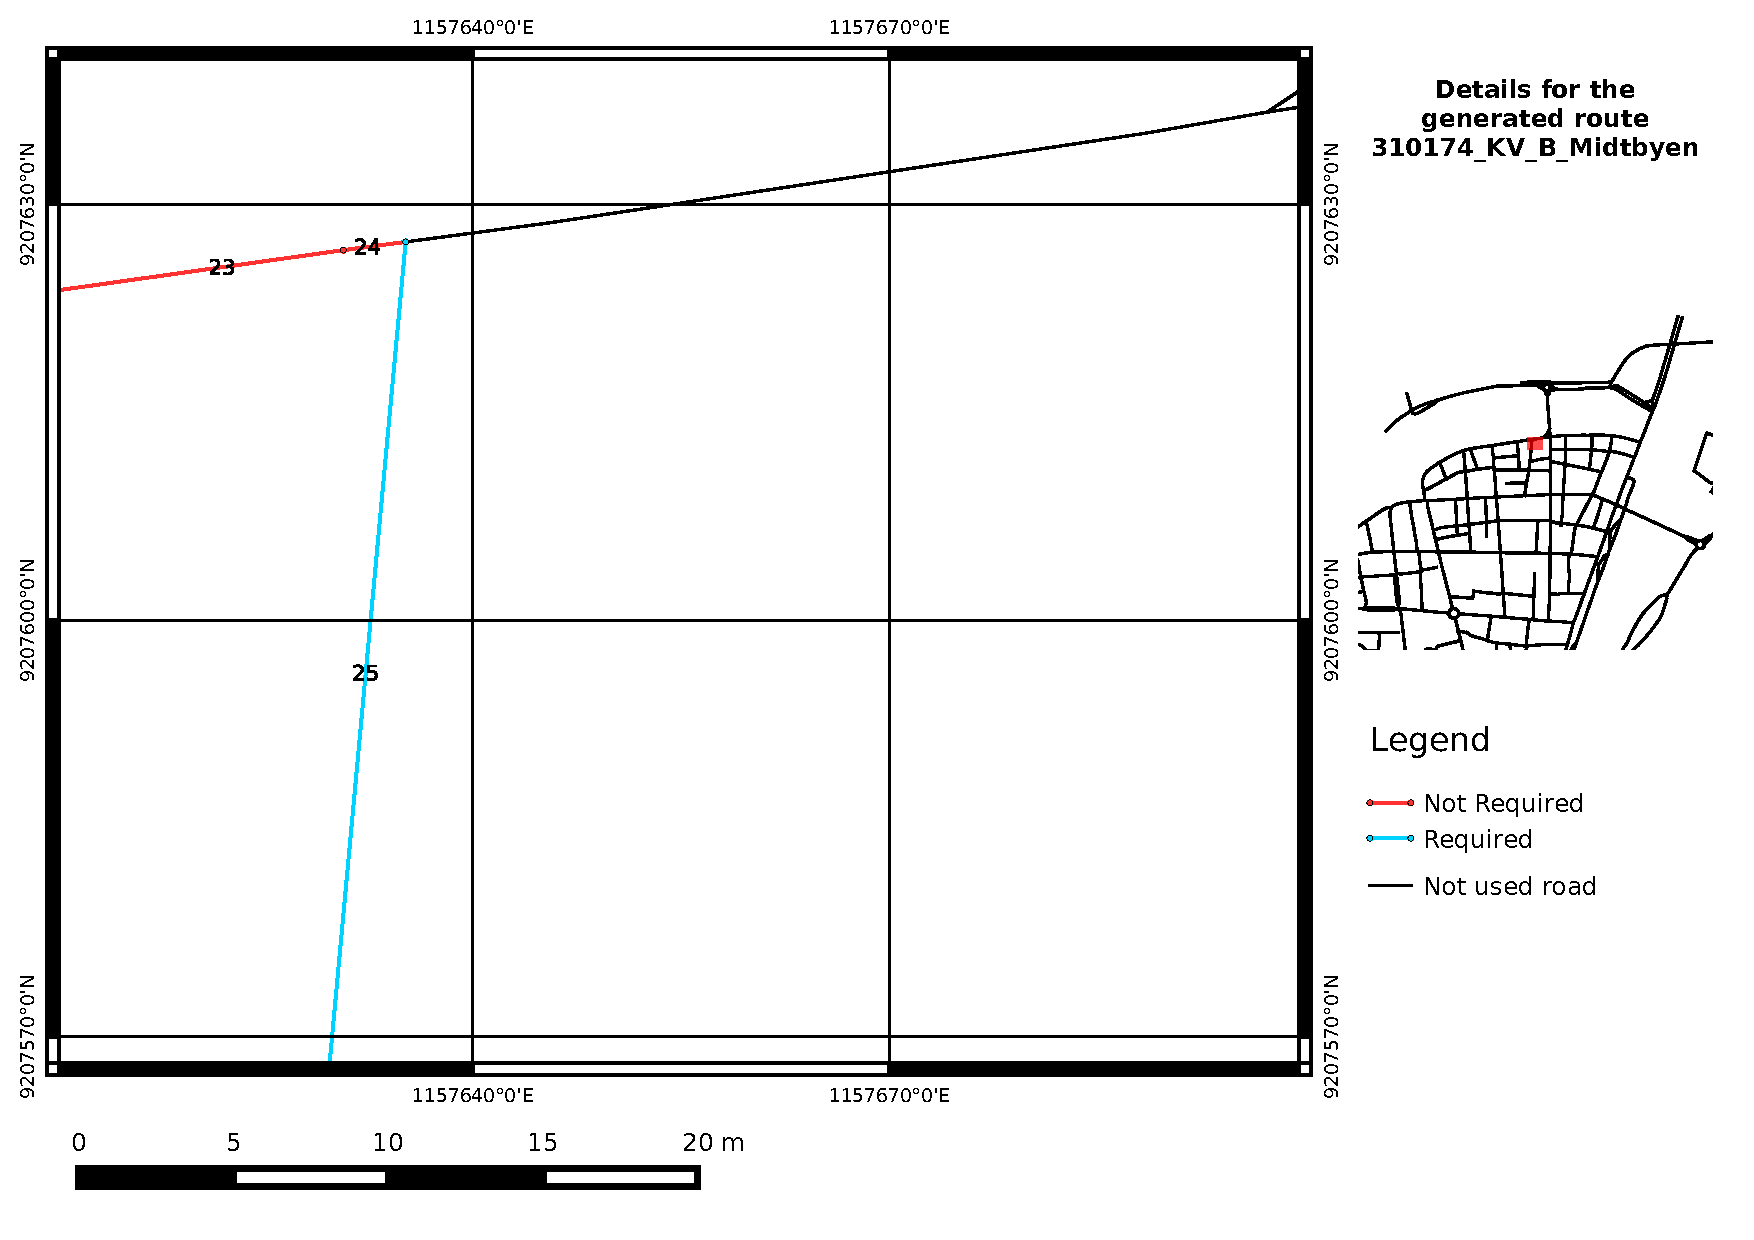
\includepdf[landscape=true,pages={-},pagecommand={\pagestyle{fancy}},height=\textwidth]{figures/Routes/DetailedMaps-atlases/2015-06-23-final_detailed_atlas_for_KV_B_midtbyen.pdf}
% \end{landscape}

% section detailed_generated_map_for_route_310174_kv_b (end)

\section{Detailed Generated Map for Route 310179\_KV\_H} % (fold)
\label{sec:detailed_generated_map_for_route_310179_kv_h}

% \begin{landscape}
% \begin{figure}[thbp]
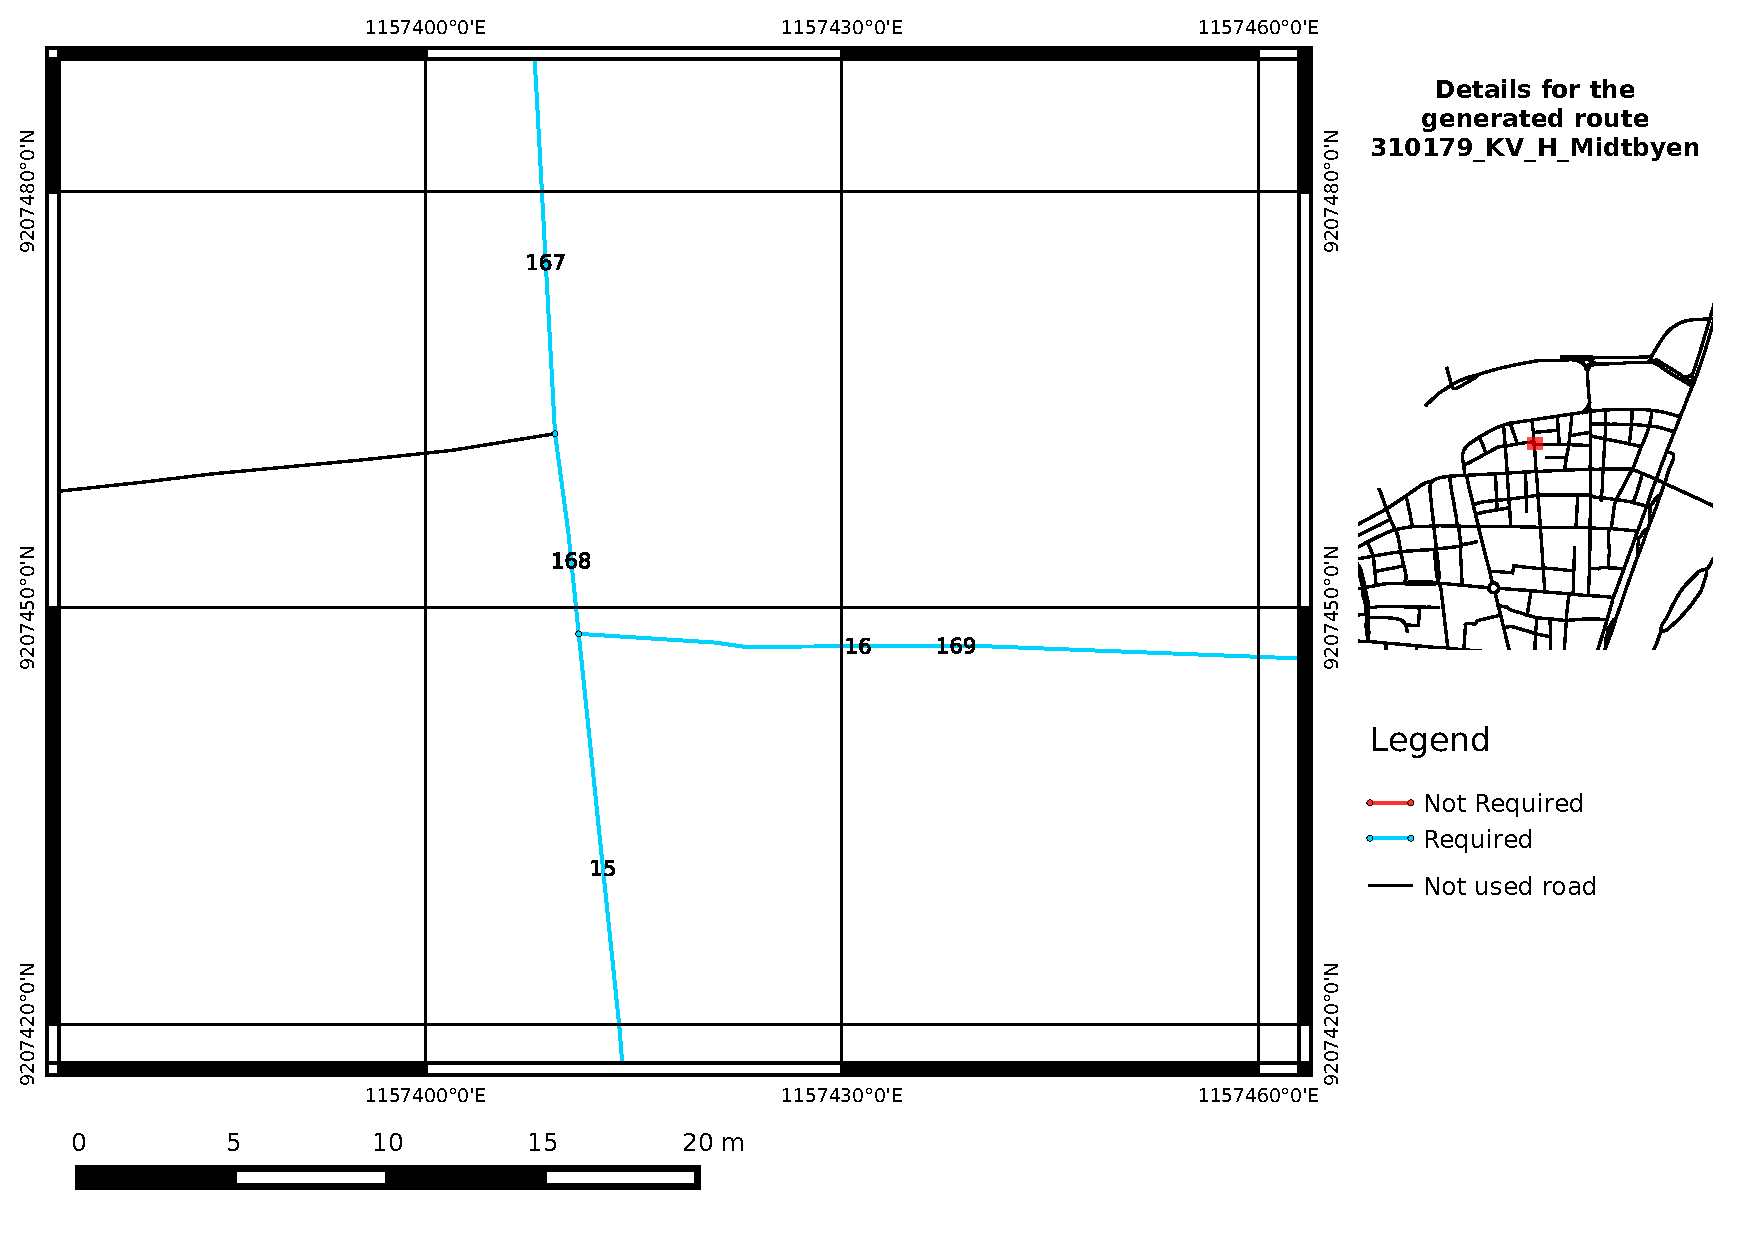
\includepdf[landscape=true,pages={-},pagecommand={\pagestyle{fancy}},height=\textwidth]{figures/Routes/DetailedMaps-atlases/2015-06-23-final_detailed_atlas_for_KV_H_midtbyen.pdf}
% 	\caption{Mutation - Average Standard Deviation}
% 	\label{fig:ctmasd}
% \end{figure}
% \end{landscape}

% section detailed_generated_map_for_route_310179_kv_h (end)

% chapter detailed_maps_for_the_generated_routes (end)
